% Plain-language review document (explaneat plain-language review), v5.
\documentclass[a4paper,10pt]{article}
\usepackage[margin=1.8cm]{geometry}
\usepackage{amsmath}
\usepackage{amssymb}
\usepackage{booktabs}
\usepackage{tabularx}
\usepackage{graphicx}
\usepackage[table,usenames,dvipsnames]{xcolor}
\usepackage{tikz}
\usetikzlibrary{arrows.meta,fit,backgrounds,positioning,calc}
\usetikzlibrary{shapes.geometric}
\usepackage{longtable}
\usepackage{pdflscape}
\usepackage{float}
\usepackage[font=small,labelfont=bf]{caption}
\usepackage{array}
\usepackage[unicode=true,hidelinks]{hyperref}
\setcounter{tocdepth}{3}
\setcounter{secnumdepth}{3}
% Review markers, copied from dissertation.tex (7 Nov 2026) for standalone builds.
\newif\ifreviewmarks
\reviewmarkstrue
\newcommand{\reviewrule}{\noindent{\color{BrickRed}\rule{\linewidth}{0.8pt}}}
\newenvironment{drafted}[1][]{%
  \ifreviewmarks\par\addvspace{\medskipamount}\reviewrule\par\nopagebreak
  \noindent{\color{BrickRed}\sffamily\footnotesize\textbf{Thesis Draft}\quad #1\hfill review}\par\nopagebreak\smallskip\fi}{%
  \ifreviewmarks\par\smallskip\noindent{\color{BrickRed}\sffamily\footnotesize end of thesis draft}\par\nopagebreak\reviewrule\par\medskip\fi}
\newcommand{\figreview}[1]{\ifreviewmarks\par\smallskip{\color{NavyBlue}\sffamily\footnotesize\textbf{Figure note:} #1}\par\fi}
\begin{document}
\begin{center}{\Large\bfseries Plain-language explanation: heart-s5-c3\par}\vspace{2mm}{\small AI-assisted drafts for review. Nothing here has been verified by a person.\par}\end{center}
\noindent\textbf{How to read this.} Explanations are built up but read down: the summary first, then each part from the whole model down, in plain words, each sentence followed by the claims it rests on (C01, C02, \ldots; every cited claim was computed on the model and checked). Numbers are changes in predicted risk for a typical patient. The technical record (original hypotheses, formulas, evidence tables with the test check, ranges and n) is at the end. The text describes what the model does, not the world; whether it is plausible is for the reviewer to judge.
\par\medskip\noindent\textbf{What changed in v5e (figures).} v5e: every diagram is a numbered figure with a caption (list of figures after the contents) and the text refers to it; the whole-network figure has its own landscape page, scaled to the page, with a short caption and its description in the text; an input used by several parts is drawn under each of them (same input, repeated for readability, dotted outline); and an appendix figure shows the trained network before any explanation (no parts, no splits).
\par\medskip\noindent\textbf{What changed in v5c (tables and diagrams).} v5c: the evidence tables are landscape, compact and shaded by row, with the header repeated on every page (longtable and pdflscape, used in this review PDF only; the thesis preamble has neither). In the diagrams each input is drawn once, in a shared row along the bottom (the explanation's split copies of an input are listed in the technical detail instead), every cluster has one output rectangle with its plain name, the inputs that feed the output directly meet in a drawn 'sum', and a one-line legend explains the edges.
\par\medskip\noindent\textbf{What changed in v5b (diagrams).} v5b uses one grouping everywhere, the annotation hierarchy: the summary's diagram is the same picture as the whole model's section, and a part that is itself a weighted sum (blood pressure with cholesterol) is a part of its own, described as one that adds up, so the text counts three parts throughout; the lint checks every 'N parts' against the hierarchy. A full-structure diagram follows the summary: every node and connection, nested by part, with the inputs that feed the output directly in their own cluster and the unused input columns listed. Each section from the top down adds its own region of that diagram, with stubs for connections from or to other parts; each connection is drawn in exactly one section. The gate's text now says that it lowers the risk for the patients it acts on, and that more vessels and higher cholesterol take that lowering away; its vessel statements are one per group.
\par\medskip\noindent\textbf{What changed in v5 (read down).} v5 reads the explanation down. The summary (one line, a diagram, one paragraph per block) is as in v4, except that the paragraph on what adds up is split into protective items, risk-raising items and rare results, and an input that also feeds a part is quoted with its direct contribution only (the rest is in that part's paragraph). Then the document walks the annotation hierarchy from the whole model down: for each part a plain hypothesis (what it does for the prediction), plain evidence (what was checked and what it showed; for a part made of others, what they are and how they combine), a diagram one level down and where to read on. The original hypotheses, closed forms and evidence tables are in 'Technical detail' at the end. Statements about structure (what a part is made of, a copy of another part, a formula that reproduces it) are now claims of their own, checked on the graph and the data.
\par\medskip\noindent\textbf{v4.} v4 follows the structure of the explanation. The summary opens with one line and a diagram at the same grouping, then gives one paragraph per top-level block of the annotation hierarchy: one for everything that adds up independently (the inputs that feed the model score directly, and parts that are a weighted sum), and one for each part that combines its inputs in another way: what it combines, how, and for whom. 'Parts in detail' follows the hierarchy below that, with a diagram one level down for each part that contains others. The prose no longer says 'clearly', 'slightly', 'consistently' or 'on the training data only': the numbers carry it, and the test check, the ranges and n stay in the evidence tables. Only genuinely small groups are marked, with their n. The lint rejects the confidence words and checks the block structure.
\tableofcontents
\listoffigures
\clearpage
\begin{drafted}[plain-language layer: heart-s5-c3]
\section{heart-s5-c3}
\noindent{\small Genome \texttt{96fb45fb-972d-4aaa-b6d5-01fc63fbc4e6}, explanation \texttt{1b3f669d-9fb5-4126-b6e4-35535db7b3b1}. Split: train primary (n=242), test as a check (n=61). Claims: 36, verified 33, not supported 3.\par}
\noindent{\small\textcolor{BrickRed}{AI-assisted draft for review (unverified)}\par}\smallskip
\noindent{\footnotesize Reference (typical) patient: the typical patient: the median training patient for every number and the most common training category for every category (not a real patient). age: 56 years; ca: 0 vessels; chol: 240 mg/dL (6.2 mmol/L); cp: no chest pain (asymptomatic); exang: no chest pain on exercise; fbs: fasting blood sugar of 120 mg/dL or less; oldpeak: 0.8 mm; restecg: a normal resting ECG; sex: male; slope: an upsloping ST segment; thal: a normal thallium scan; thalach: 152 beats per minute; trestbps: 130 mm Hg. Predicted risk of heart disease: 18\%.\par}
\subsection{Summary}
\noindent For a typical patient (a 56-year-old man with no chest pain symptoms and median test results) the model predicts a risk of heart disease of about 18\%; it adds up most of its inputs independently, and two parts add to that sum: a signal from ST depression on exercise and the resting ECG that acts on 105 of 242 training patients, and an age term that acts on 148.\,{\scriptsize\textcolor{NavyBlue}{[C25, C30, C34]}} Figure~\ref{fig:hearts5c3:summary} shows the model at this level: one box per paragraph below.
\par\medskip\noindent\fbox{\begin{minipage}{0.96\linewidth}\small\textbf{How to read the diagrams.} Edge colour is the sign of that one connection: blue positive, red negative; thicker is a larger weight. The outline and arrow on an input (and on a part's output box) is its overall effect on the final prediction, read from the verified claims: orange and up arrow raises it, teal and down arrow lowers it, grey and double arrow depends (it goes both ways, or differs between levels). A negative connection into a part that itself raises the prediction means that input lowers the prediction; through a hinge the overall effect can only be read from the claims, not from the edges. Up arrow means towards heart disease; down arrow, away from it. A double outline marks an input (or a part's output) that acts at a fixed rate everywhere: it adds the same amount to the score per unit, so it is explained by its rate alone (see 'Linear factors'); a dashed double outline, at a fixed rate on the observed data. The normal outline is an input whose effect switches on and off somewhere. For example, ST depression has a positive connection into 'ST depression signal', a part that raises the predicted risk of heart disease, so ST depression raises it.\end{minipage}}\par\medskip
\begin{figure}[H]\centering
\resizebox{!}{\ifdim\height>0.5\textheight 0.5\textheight\else\height\fi}{%
\resizebox{\ifdim\width>\linewidth\linewidth\else\width\fi}{!}{%
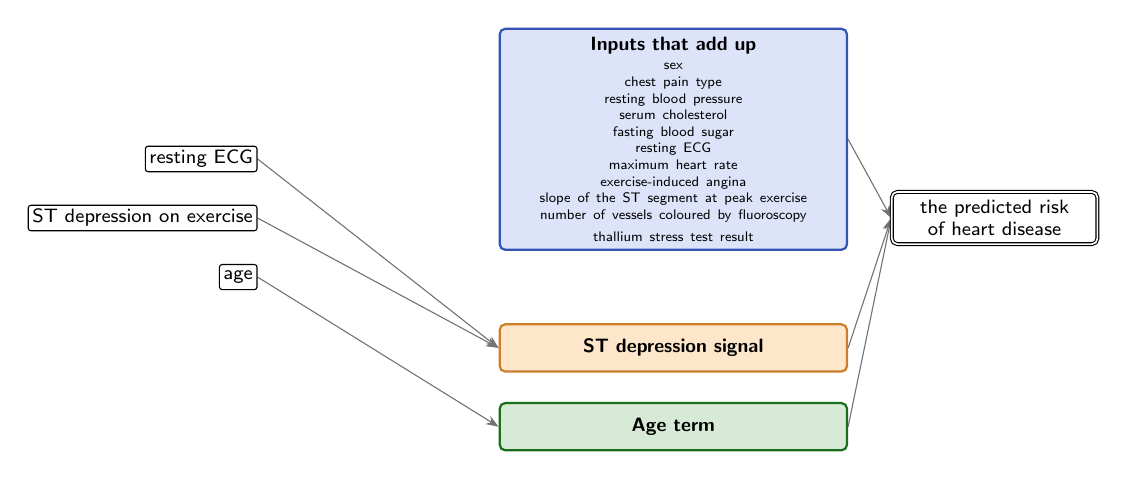
\begin{tikzpicture}[
  font=\sffamily\scriptsize, >={Stealth[length=1.6mm]},
  inp/.style={draw, rounded corners=1pt, fill=white, inner sep=1.5pt, minimum height=3.2mm, anchor=east},
  abox/.style={draw, thick, rounded corners=2pt, align=center, inner sep=3pt, minimum height=6mm, text width=42mm},
  outp/.style={draw, double, rounded corners=2pt, fill=white, align=center, inner sep=3pt, text width=24mm},
  agg/.style={draw=black!55},
]
\node[inp] (i0) at (0,0.75) {resting ECG};
\node[inp] (i1) at (0,-0.0) {ST depression on exercise};
\node[inp] (i2) at (0,-0.75) {age};
\node[abox, fill=RoyalBlue!18, draw=RoyalBlue!80!black] (b0) at (5.28,1.0) {\textbf{Inputs that add up}\\[1pt]{\tiny sex\\ chest pain type\\ resting blood pressure\\ serum cholesterol\\ fasting blood sugar\\ resting ECG\\ maximum heart rate\\ exercise-induced angina\\ slope of the ST segment at peak exercise\\ number of vessels coloured by fluoroscopy\\ thallium stress test result}};
\node[abox, fill=BurntOrange!18, draw=BurntOrange!80!black] (b1) at (5.28,-1.65) {\textbf{ST depression signal}};
\node[abox, fill=ForestGreen!18, draw=ForestGreen!80!black] (b2) at (5.28,-2.65) {\textbf{Age term}};
\node[outp] (out) at (9.36,0) {the predicted risk of heart disease};
\begin{scope}[on background layer]
\draw[->, agg] (b0.east) -- (out.west);
\draw[->, agg, thin] (i0.east) -- (b1.west);
\draw[->, agg, thin] (i1.east) -- (b1.west);
\draw[->, agg] (b1.east) -- (out.west);
\draw[->, agg, thin] (i2.east) -- (b2.west);
\draw[->, agg] (b2.east) -- (out.west);
\end{scope}
\end{tikzpicture}}}%
\caption{The model at the level of the summary: one box per part.}
\label{fig:hearts5c3:summary}
\end{figure}
\paragraph{Inputs that add up.} \par\noindent\textit{Lowering the risk.}  These add up independently, and these lower the risk: being a woman takes a typical patient's predicted risk from about 18\% to about 2\%, typical angina to about 2\%, non-anginal chest pain to about 4\% and atypical angina to about 10\%; fasting blood sugar above 120 mg/dL lowers it to about 9\%; and a higher maximum heart rate lowers it steadily, from about 23\% at 118 to about 15\% at 175 beats per minute.\,{\scriptsize\textcolor{NavyBlue}{[C10, C09, C11, C15, C12, C14]}} \par\noindent\textit{Raising the risk.}  Each extra vessel coloured by fluoroscopy adds about the same, from about 18\% at 0 to about 86\% at 2 vessels, flattening out near the top because the predicted risk cannot go much higher; a flat rather than upsloping ST segment raises it to about 56\%, a reversible defect on the thallium scan to about 38\% and chest pain brought on by exercise to about 35\%; higher cholesterol raises it steadily, from about 11\% at 193 mg/dL to about 33\% at 308 mg/dL, and higher resting blood pressure steadily, from about 12\% at 110 mm Hg to about 30\% at 155 mm Hg.\,{\scriptsize\textcolor{NavyBlue}{[C01, C04, C06, C08, C05, C07]}} Through this sum alone, a resting ECG other than normal raises it from about 18\% to about 24\%; the resting ECG also acts through the ST depression signal (below).\,{\scriptsize\textcolor{NavyBlue}{[C16]}} \par\noindent\textit{Rare results.}  Some rarer results also count (the model has little data on this, n = 2 to 17): a thallium result coded 4 raises the risk to about 79\%, a fixed defect on the thallium scan lowers it to about 9\%, and a downsloping ST segment leaves it at about 19\%.\,{\scriptsize\textcolor{NavyBlue}{[C02, C13, C19]}}
\paragraph{ST depression signal.} This part reads ST depression on exercise and the resting ECG, and acts on 105 of 242 training patients, 66 of whom had heart disease; for the typical patient it acts on, the predicted risk is about 76\% without it and about 91\% with it.\,{\scriptsize\textcolor{NavyBlue}{[C30]}} Through it, more ST depression adds nothing until about 0.5 mm, then raises the predicted risk steadily: for a typical patient from about 16\% at 0 mm to about 60\% at 2.8 mm.\,{\scriptsize\textcolor{NavyBlue}{[C26]}} ST depression counts more with a normal resting ECG, nothing until about 0.5 mm and then steadily, from about 16\% to about 60\%, against about 21\% to about 48\% with any other resting ECG.\,{\scriptsize\textcolor{NavyBlue}{[C28]}} Through it, a resting ECG other than normal lowers a typical patient's risk from about 18\% to about 16\%.\,{\scriptsize\textcolor{NavyBlue}{[C27]}}
\paragraph{Age term.} This part acts on 148 of 242 training patients, 81 of whom had heart disease; for the typical patient it acts on, the predicted risk is about 91\% without it and about 92\% with it.\,{\scriptsize\textcolor{NavyBlue}{[C34]}} Through it, age adds nothing until about 53 years, then raises the risk steadily, for a typical patient from about 18\% at 42 to about 19\% at 66 years.\,{\scriptsize\textcolor{NavyBlue}{[C32, C33]}}
\paragraph{The whole network.} Figure~\ref{fig:hearts5c3:overview} (next page, landscape) draws every unit and connection of the explained model, nested by part: shaded clusters are the parts of the model and darker boxes the parts inside them; circles are hidden units (h1, h2, \ldots); each cluster's rectangle is its output, and a dashed `sum' stands for an addition the next unit does (drawn, not a unit of the model); the hexagon is the model's output. An input used by several parts is drawn under each of them (same label, dotted outline, the first copy marked with the number of copies): it is the same input, repeated for readability. Not used by the model (input columns with no connection): male, atypical angina, sugar above 120, ST-T abnormal ECG, LVH on ECG, no exercise pain, flat ST.
\begin{landscape}
\begin{figure}[p]\centering
\resizebox{\linewidth}{!}{%
\definecolor{netup}{HTML}{D95F02}\definecolor{netdown}{HTML}{1B9E77}\definecolor{netmixed}{HTML}{7F7F7F}%
\begin{tikzpicture}[
  font=\sffamily\scriptsize, >={Stealth[length=1.4mm]},
  inp/.style={draw, circle, fill=white, minimum size=3.2mm, inner sep=0pt},
  hid/.style={draw, circle, fill=white, minimum size=5.2mm, inner sep=0.5pt, font=\sffamily\tiny},
  exitbox/.style={draw, thick, rectangle, fill=white, align=center, text width=17mm, minimum height=5mm, inner sep=1.5pt, font=\sffamily\tiny},
  sumbox/.style={draw, thick, dashed, rectangle, fill=white, align=center, text width=17mm, minimum height=5mm, inner sep=1.5pt, font=\sffamily\tiny},
  outp/.style={draw, thick, regular polygon, regular polygon sides=6, fill=white, minimum size=10mm, inner sep=0pt, font=\sffamily\tiny, align=center},
  stub/.style={draw, dashed, rounded corners=2pt, fill=white, align=center, inner sep=2pt, font=\sffamily\tiny, text width=15mm},
  inlab/.style={font=\sffamily\tiny, align=center, text width=15mm, inner sep=1pt, fill=white, fill opacity=0.8, text opacity=1},
  wpos/.style={draw=NavyBlue}, wneg/.style={draw=BrickRed}, wagg/.style={draw=black!45, line width=1.2pt},
  wmix/.style={draw=Plum},
]
\node[outp] (n0) at (10.34,7.5) {heart disease};
\node[exitbox] (n1987) at (19.78,1.9) {Age term $\uparrow$};
\node[hid] (n204) at (15.24,1.9) {h1};
\node[hid] (n290) at (15.24,4.6) {h2};
\node[hid] (n3487) at (15.24,3.25) {h4};
\node[sumbox] (ncsumxxannx27) at (15.24,5.95) {sum: ST depression signal $\uparrow$};
\node[sumbox] (nxxsumxx) at (5.85,1.9) {sum: Inputs that add up};
\node[inp, draw=netdown, very thick] (ninxxsexx0xxadditive) at (2.7,-2.1) {};
\path (ninxxsexx0xxadditive.south) node[inlab, anchor=north] (labninxxsexx0xxadditive) {female $\downarrow$};
\node[inp, draw=netdown, very thick] (ninxxcpx1xxadditive) at (9.0,-1.05) {};
\path (ninxxcpx1xxadditive.south) node[inlab, anchor=north] (labninxxcpx1xxadditive) {typical angina $\downarrow$};
\node[inp, draw=netdown, very thick] (ninxxcpx3xxadditive) at (5.4,-1.05) {};
\path (ninxxcpx3xxadditive.south) node[inlab, anchor=north] (labninxxcpx3xxadditive) {non-anginal pain $\downarrow$};
\node[inp, draw=netup, very thick] (ninxxcpx4xxadditive) at (4.5,-2.1) {};
\path (ninxxcpx4xxadditive.south) node[inlab, anchor=north] (labninxxcpx4xxadditive) {no chest pain $\uparrow$};
\node[inp, draw=netup, very thick] (ninxxtrestbpsxxadditive) at (0.9,0.0) {};
\path (ninxxtrestbpsxxadditive.south) node[inlab, anchor=north] (labninxxtrestbpsxxadditive) {blood pressure $\uparrow$};
\node[inp, draw=netup, very thick] (ninxxcholxxadditive) at (0.9,-2.1) {};
\path (ninxxcholxxadditive.south) node[inlab, anchor=north] (labninxxcholxxadditive) {cholesterol $\uparrow$};
\node[inp, draw=netup, very thick] (ninxxfbsx0xxadditive) at (8.1,0.0) {};
\path (ninxxfbsx0xxadditive.south) node[inlab, anchor=north] (labninxxfbsx0xxadditive) {sugar 120 or less $\uparrow$};
\node[inp, draw=netdown, very thick] (ninxxthalachxxadditive) at (4.5,0.0) {};
\path (ninxxthalachxxadditive.south) node[inlab, anchor=north] (labninxxthalachxxadditive) {max heart rate $\downarrow$};
\node[inp, draw=netup, very thick] (ninxxexangx1xxadditive) at (2.7,0.0) {};
\path (ninxxexangx1xxadditive.south) node[inlab, anchor=north] (labninxxexangx1xxadditive) {exercise pain $\uparrow$};
\node[inp, draw=netdown, very thick] (ninxxslopex1xxadditive) at (9.9,0.0) {};
\path (ninxxslopex1xxadditive.south) node[inlab, anchor=north] (labninxxslopex1xxadditive) {upsloping ST $\downarrow$};
\node[inp, draw=netup, very thick] (ninxxslopex3xxadditive) at (1.8,-1.05) {};
\path (ninxxslopex3xxadditive.south) node[inlab, anchor=north] (labninxxslopex3xxadditive) {downsloping ST $\uparrow$};
\node[inp, draw=netup, very thick] (ninxxcaxxadditive) at (10.8,-1.05) {};
\path (ninxxcaxxadditive.south) node[inlab, anchor=north] (labninxxcaxxadditive) {vessels $\uparrow$};
\node[inp, draw=netmixed, very thick] (ninxxthalx3xxadditive) at (6.3,-2.1) {};
\path (ninxxthalx3xxadditive.south) node[inlab, anchor=north] (labninxxthalx3xxadditive) {normal thallium $\updownarrow$};
\node[inp, draw=netup, very thick] (ninxxthalx4xxadditive) at (8.1,-2.1) {};
\path (ninxxthalx4xxadditive.south) node[inlab, anchor=north] (labninxxthalx4xxadditive) {thallium code 4 $\uparrow$};
\node[inp, draw=netdown, very thick] (ninxxthalx6xxadditive) at (3.6,-1.05) {};
\path (ninxxthalx6xxadditive.south) node[inlab, anchor=north] (labninxxthalx6xxadditive) {fixed defect $\downarrow$};
\node[inp, draw=netup, very thick] (ninxxthalx7xxadditive) at (7.2,-1.05) {};
\path (ninxxthalx7xxadditive.south) node[inlab, anchor=north] (labninxxthalx7xxadditive) {reversible defect $\uparrow$};
\node[inp, draw=netup, very thick] (ninxxoldpeakxxannx27) at (14.34,0.0) {};
\path (ninxxoldpeakxxannx27.south) node[inlab, anchor=north] (labninxxoldpeakxxannx27) {ST depression $\uparrow$};
\node[inp, draw=netup, very thick] (ninxxagexxannx28) at (19.78,0.0) {};
\path (ninxxagexxannx28.south) node[inlab, anchor=north] (labninxxagexxannx28) {age $\uparrow$};
\node[inp, densely dotted, thick, draw=netdown, very thick] (ninxxrestecgx0xxadditive) at (6.3,0.0) {};
\path (ninxxrestecgx0xxadditive.south) node[inlab, anchor=north] (labninxxrestecgx0xxadditive) {normal ECG ($\times$2) $\downarrow$};
\node[inp, densely dotted, thick, draw=netup, very thick] (ninxxrestecgx0xxannx27) at (16.14,0.0) {};
\path (ninxxrestecgx0xxannx27.south) node[inlab, anchor=north] (labninxxrestecgx0xxannx27) {normal ECG $\uparrow$};
\begin{scope}[on background layer]
\node[fit=(nxxsumxx) , inner sep=8pt, rounded corners=5pt, fill=RoyalBlue!10, draw=RoyalBlue!45] (clu0) {};
\node[fit=(n204) (n290) (n3487) (ncsumxxannx27) , inner sep=8pt, rounded corners=5pt, fill=BurntOrange!10, draw=BurntOrange!45] (clu1) {};
\node[fit=(n1987) , inner sep=8pt, rounded corners=5pt, fill=ForestGreen!10, draw=ForestGreen!45] (clu2) {};
\draw[->, wneg, line width=0.61pt] (ninxxsexx0xxadditive) -- (nxxsumxx);
\draw[->, wneg, line width=0.42pt] (ninxxcpx1xxadditive) -- (nxxsumxx);
\draw[->, wneg, line width=0.40pt] (ninxxcpx3xxadditive) -- (nxxsumxx);
\draw[->, wpos, line width=0.37pt] (ninxxcpx4xxadditive) -- (nxxsumxx);
\draw[->, wpos, line width=0.42pt] (ninxxtrestbpsxxadditive) -- (nxxsumxx);
\draw[->, wpos, line width=0.44pt] (ninxxcholxxadditive) -- (nxxsumxx);
\draw[->, wpos, line width=0.35pt] (ninxxfbsx0xxadditive) -- (nxxsumxx);
\draw[->, wneg, line width=0.32pt] (ninxxthalachxxadditive) -- (nxxsumxx);
\draw[->, wpos, line width=0.40pt] (ninxxexangx1xxadditive) -- (nxxsumxx);
\draw[->, wneg, line width=0.56pt] (ninxxslopex1xxadditive) -- (nxxsumxx);
\draw[->, wneg, line width=0.40pt] (ninxxslopex3xxadditive) -- (nxxsumxx);
\draw[->, wpos, line width=0.77pt] (ninxxcaxxadditive) -- (nxxsumxx);
\draw[->, wneg, line width=0.41pt] (ninxxthalx3xxadditive) -- (nxxsumxx);
\draw[->, wpos, line width=0.31pt] (ninxxthalx4xxadditive) -- (nxxsumxx);
\draw[->, wneg, line width=0.40pt] (ninxxthalx6xxadditive) -- (nxxsumxx);
\draw[->, wpos, line width=0.26pt] (ninxxthalx7xxadditive) -- (nxxsumxx);
\draw[->, wpos, line width=0.27pt] (n204) -- (ncsumxxannx27);
\draw[->, wpos, line width=0.33pt] (n290) -- (ncsumxxannx27);
\draw[->, wpos, line width=0.28pt] (n1987) -- (n0);
\draw[->, wpos, line width=1.13pt] (ninxxoldpeakxxannx27) -- (n204);
\draw[->, wpos, line width=0.56pt] (ninxxagexxannx28) -- (n1987);
\draw[->, wpos, line width=0.60pt] (n204) -- (n290);
\draw[->, wpos, line width=0.58pt] (n204) -- (n3487);
\draw[->, wpos, line width=0.55pt] (n3487) -- (n290);
\draw[->, wneg, line width=0.32pt] (ninxxrestecgx0xxadditive) -- (nxxsumxx);
\draw[->, wpos, line width=0.59pt] (ninxxrestecgx0xxannx27) -- (n204);
\draw[->, wagg] (ncsumxxannx27) -- (n0);
\draw[->, wagg] (nxxsumxx) -- (n0);
\end{scope}
\node[font=\sffamily\scriptsize\bfseries, text=RoyalBlue!55!black, anchor=south west, inner sep=1pt, fill=white, fill opacity=0.85, text opacity=1] at (clu0.north west) {Inputs that add up};
\node[font=\sffamily\scriptsize\bfseries, text=BurntOrange!55!black, anchor=south west, inner sep=1pt, fill=white, fill opacity=0.85, text opacity=1] at (clu1.north west) {ST depression signal};
\node[font=\sffamily\scriptsize\bfseries, text=ForestGreen!55!black, anchor=south west, inner sep=1pt, fill=white, fill opacity=0.85, text opacity=1] at (clu2.north west) {Age term};
\end{tikzpicture}}%
\caption{Every unit and connection of the explained model, nested by part. Blue: positive weight (raises the score); red: negative weight (lowers it); thicker: larger weight. Orange outline and up arrow: raises the final prediction; teal and down arrow: lowers it; grey and double arrow: depends.}
\label{fig:hearts5c3:overview}
\end{figure}
\end{landscape}
\paragraph{Worth checking against what is known.} Worth checking: the model treats fasting blood sugar above 120 mg/dL as lowering the risk of heart disease (for a typical patient from about 18\% to about 9\%).\,{\scriptsize\textcolor{NavyBlue}{[C12]}} Worth checking: patients with typical angina get the lowest predicted risk of all chest pain types, below patients with no chest pain symptoms.\,{\scriptsize\textcolor{NavyBlue}{[C09, C11, C15]}} Worth checking: the model treats a fixed defect on the thallium scan as lowering the risk compared with a normal scan, from only 15 training patients.\,{\scriptsize\textcolor{NavyBlue}{[C13]}} Worth checking: the model gives a higher predicted risk to the 2 training patients whose thallium result is coded 4, a code the dataset documentation does not define.\,{\scriptsize\textcolor{NavyBlue}{[C02]}} Worth checking: ST depression on exercise raises the predicted risk more when the resting ECG is normal than when it is not.\,{\scriptsize\textcolor{NavyBlue}{[C28]}}
\subsection{The model, read from the top down}
\noindent{\small Each part of the explanation in turn, from the whole model down to the smallest parts: what it does for the prediction (hypothesis), what was checked (evidence), a diagram one level down, and where to read on. The technical record of each part is in ``Technical detail'' at the end.\par}
\subsubsection{The whole model}\label{rd:ann29}
\noindent{\small Figure~\ref{fig:hearts5c3:parts-ann29} shows what feeds this part; Figure~\ref{fig:hearts5c3:units-ann29} its units and every connection into them (dashed boxes: connections from or to other parts, drawn in their own sections).\par}
\begin{figure}[H]\centering
\resizebox{!}{\ifdim\height>0.5\textheight 0.5\textheight\else\height\fi}{%
\resizebox{\ifdim\width>\linewidth\linewidth\else\width\fi}{!}{%
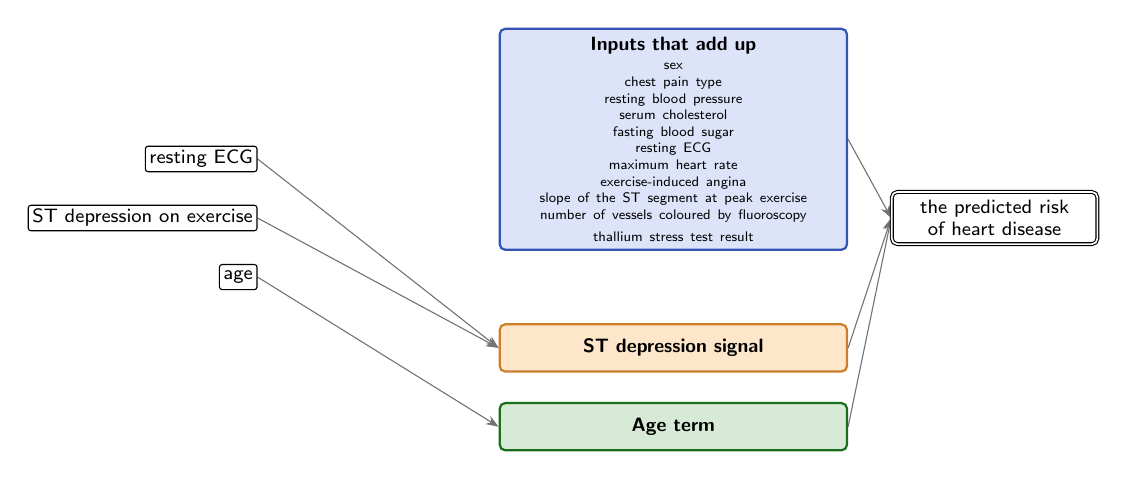
\begin{tikzpicture}[
  font=\sffamily\scriptsize, >={Stealth[length=1.6mm]},
  inp/.style={draw, rounded corners=1pt, fill=white, inner sep=1.5pt, minimum height=3.2mm, anchor=east},
  abox/.style={draw, thick, rounded corners=2pt, align=center, inner sep=3pt, minimum height=6mm, text width=42mm},
  outp/.style={draw, double, rounded corners=2pt, fill=white, align=center, inner sep=3pt, text width=24mm},
  agg/.style={draw=black!55},
]
\node[inp] (i0) at (0,0.75) {resting ECG};
\node[inp] (i1) at (0,-0.0) {ST depression on exercise};
\node[inp] (i2) at (0,-0.75) {age};
\node[abox, fill=RoyalBlue!18, draw=RoyalBlue!80!black] (b0) at (5.28,1.0) {\textbf{Inputs that add up}\\[1pt]{\tiny sex\\ chest pain type\\ resting blood pressure\\ serum cholesterol\\ fasting blood sugar\\ resting ECG\\ maximum heart rate\\ exercise-induced angina\\ slope of the ST segment at peak exercise\\ number of vessels coloured by fluoroscopy\\ thallium stress test result}};
\node[abox, fill=BurntOrange!18, draw=BurntOrange!80!black] (b1) at (5.28,-1.65) {\textbf{ST depression signal}};
\node[abox, fill=ForestGreen!18, draw=ForestGreen!80!black] (b2) at (5.28,-2.65) {\textbf{Age term}};
\node[outp] (out) at (9.36,0) {the predicted risk of heart disease};
\begin{scope}[on background layer]
\draw[->, agg] (b0.east) -- (out.west);
\draw[->, agg, thin] (i0.east) -- (b1.west);
\draw[->, agg, thin] (i1.east) -- (b1.west);
\draw[->, agg] (b1.east) -- (out.west);
\draw[->, agg, thin] (i2.east) -- (b2.west);
\draw[->, agg] (b2.east) -- (out.west);
\end{scope}
\end{tikzpicture}}}%
\caption{The whole model: what feeds it, one level down.}
\label{fig:hearts5c3:parts-ann29}
\end{figure}
\begin{figure}[H]\centering
\resizebox{\ifdim\width>\linewidth\linewidth\else\width\fi}{!}{%
\definecolor{netup}{HTML}{D95F02}\definecolor{netdown}{HTML}{1B9E77}\definecolor{netmixed}{HTML}{7F7F7F}%
\begin{tikzpicture}[
  font=\sffamily\scriptsize, >={Stealth[length=1.4mm]},
  inp/.style={draw, circle, fill=white, minimum size=3.2mm, inner sep=0pt},
  hid/.style={draw, circle, fill=white, minimum size=5.2mm, inner sep=0.5pt, font=\sffamily\tiny},
  exitbox/.style={draw, thick, rectangle, fill=white, align=center, text width=17mm, minimum height=5mm, inner sep=1.5pt, font=\sffamily\tiny},
  sumbox/.style={draw, thick, dashed, rectangle, fill=white, align=center, text width=17mm, minimum height=5mm, inner sep=1.5pt, font=\sffamily\tiny},
  outp/.style={draw, thick, regular polygon, regular polygon sides=6, fill=white, minimum size=10mm, inner sep=0pt, font=\sffamily\tiny, align=center},
  stub/.style={draw, dashed, rounded corners=2pt, fill=white, align=center, inner sep=2pt, font=\sffamily\tiny, text width=15mm},
  inlab/.style={font=\sffamily\tiny, align=center, text width=15mm, inner sep=1pt, fill=white, fill opacity=0.8, text opacity=1},
  wpos/.style={draw=NavyBlue}, wneg/.style={draw=BrickRed}, wagg/.style={draw=black!45, line width=1.2pt},
  wmix/.style={draw=Plum},
]
\node[outp] (n0) at (8.42,3.45) {heart disease};
\node[inp, draw=netdown, very thick] (ninxxsexx0) at (2.7,-2.1) {};
\path (ninxxsexx0.south) node[inlab, anchor=north] (labninxxsexx0) {female $\downarrow$};
\node[sumbox] (nxxsumxx) at (5.85,1.9) {sum: Inputs that add up};
\node[inp, draw=netdown, very thick] (ninxxcpx1) at (9.0,-1.05) {};
\path (ninxxcpx1.south) node[inlab, anchor=north] (labninxxcpx1) {typical angina $\downarrow$};
\node[inp, draw=netdown, very thick] (ninxxcpx3) at (5.4,-1.05) {};
\path (ninxxcpx3.south) node[inlab, anchor=north] (labninxxcpx3) {non-anginal pain $\downarrow$};
\node[inp, draw=netup, very thick] (ninxxcpx4) at (4.5,-2.1) {};
\path (ninxxcpx4.south) node[inlab, anchor=north] (labninxxcpx4) {no chest pain $\uparrow$};
\node[inp, draw=netup, very thick] (ninxxtrestbps) at (0.9,0.0) {};
\path (ninxxtrestbps.south) node[inlab, anchor=north] (labninxxtrestbps) {blood pressure $\uparrow$};
\node[inp, draw=netup, very thick] (ninxxchol) at (0.9,-2.1) {};
\path (ninxxchol.south) node[inlab, anchor=north] (labninxxchol) {cholesterol $\uparrow$};
\node[inp, draw=netup, very thick] (ninxxfbsx0) at (8.1,0.0) {};
\path (ninxxfbsx0.south) node[inlab, anchor=north] (labninxxfbsx0) {sugar 120 or less $\uparrow$};
\node[inp, draw=netdown, very thick] (ninxxthalach) at (4.5,0.0) {};
\path (ninxxthalach.south) node[inlab, anchor=north] (labninxxthalach) {max heart rate $\downarrow$};
\node[inp, draw=netup, very thick] (ninxxexangx1) at (2.7,0.0) {};
\path (ninxxexangx1.south) node[inlab, anchor=north] (labninxxexangx1) {exercise pain $\uparrow$};
\node[inp, draw=netdown, very thick] (ninxxslopex1) at (9.9,0.0) {};
\path (ninxxslopex1.south) node[inlab, anchor=north] (labninxxslopex1) {upsloping ST $\downarrow$};
\node[inp, draw=netup, very thick] (ninxxslopex3) at (1.8,-1.05) {};
\path (ninxxslopex3.south) node[inlab, anchor=north] (labninxxslopex3) {downsloping ST $\uparrow$};
\node[inp, draw=netup, very thick] (ninxxca) at (10.8,-1.05) {};
\path (ninxxca.south) node[inlab, anchor=north] (labninxxca) {vessels $\uparrow$};
\node[inp, draw=netmixed, very thick] (ninxxthalx3) at (6.3,-2.1) {};
\path (ninxxthalx3.south) node[inlab, anchor=north] (labninxxthalx3) {normal thallium $\updownarrow$};
\node[inp, draw=netup, very thick] (ninxxthalx4) at (8.1,-2.1) {};
\path (ninxxthalx4.south) node[inlab, anchor=north] (labninxxthalx4) {thallium code 4 $\uparrow$};
\node[inp, draw=netdown, very thick] (ninxxthalx6) at (3.6,-1.05) {};
\path (ninxxthalx6.south) node[inlab, anchor=north] (labninxxthalx6) {fixed defect $\downarrow$};
\node[inp, draw=netup, very thick] (ninxxthalx7) at (7.2,-1.05) {};
\path (ninxxthalx7.south) node[inlab, anchor=north] (labninxxthalx7) {reversible defect $\uparrow$};
\node[stub] (nfromxxSTxdepressionxsignal) at (15.94,0.0) {from ST depression signal};
\node[stub] (nfromxxAgexterm) at (14.14,0.0) {from Age term};
\node[inp, draw=netdown, very thick] (ninxxrestecgx0) at (6.3,0.0) {};
\path (ninxxrestecgx0.south) node[inlab, anchor=north] (labninxxrestecgx0) {normal ECG $\downarrow$};
\begin{scope}[on background layer]
\node[fit=(nxxsumxx) , inner sep=8pt, rounded corners=5pt, fill=RoyalBlue!10, draw=RoyalBlue!45] (clu0) {};
\draw[->, wneg, line width=0.61pt] (ninxxsexx0) -- (nxxsumxx);
\draw[->, wneg, line width=0.42pt] (ninxxcpx1) -- (nxxsumxx);
\draw[->, wneg, line width=0.40pt] (ninxxcpx3) -- (nxxsumxx);
\draw[->, wpos, line width=0.37pt] (ninxxcpx4) -- (nxxsumxx);
\draw[->, wpos, line width=0.42pt] (ninxxtrestbps) -- (nxxsumxx);
\draw[->, wpos, line width=0.44pt] (ninxxchol) -- (nxxsumxx);
\draw[->, wpos, line width=0.35pt] (ninxxfbsx0) -- (nxxsumxx);
\draw[->, wneg, line width=0.32pt] (ninxxthalach) -- (nxxsumxx);
\draw[->, wpos, line width=0.40pt] (ninxxexangx1) -- (nxxsumxx);
\draw[->, wneg, line width=0.56pt] (ninxxslopex1) -- (nxxsumxx);
\draw[->, wneg, line width=0.40pt] (ninxxslopex3) -- (nxxsumxx);
\draw[->, wpos, line width=0.77pt] (ninxxca) -- (nxxsumxx);
\draw[->, wneg, line width=0.41pt] (ninxxthalx3) -- (nxxsumxx);
\draw[->, wpos, line width=0.31pt] (ninxxthalx4) -- (nxxsumxx);
\draw[->, wneg, line width=0.40pt] (ninxxthalx6) -- (nxxsumxx);
\draw[->, wpos, line width=0.26pt] (ninxxthalx7) -- (nxxsumxx);
\draw[->, wpos, line width=0.27pt] (nfromxxSTxdepressionxsignal) -- (n0);
\draw[->, wpos, line width=0.33pt] (nfromxxSTxdepressionxsignal) -- (n0);
\draw[->, wpos, line width=0.28pt] (nfromxxAgexterm) -- (n0);
\draw[->, wneg, line width=0.32pt] (ninxxrestecgx0) -- (nxxsumxx);
\draw[->, wagg] (nxxsumxx) -- (n0);
\end{scope}
\node[font=\sffamily\scriptsize\bfseries, text=RoyalBlue!55!black, anchor=south west, inner sep=1pt, fill=white, fill opacity=0.85, text opacity=1] at (clu0.north west) {Inputs that add up};
\end{tikzpicture}}%
\caption{The whole model: its units and every connection into them. Blue: positive weight (raises the score); red: negative weight (lowers it); thicker: larger weight. Orange outline and up arrow: raises the final prediction; teal and down arrow: lowers it; grey and double arrow: depends.}
\label{fig:hearts5c3:units-ann29}
\end{figure}
\paragraph{Hypothesis.} The model adds up its inputs into one score: the vessels coloured (each extra vessel adding about the same), the ST segment, sex and chest pain type each move the predicted risk on their own, and two parts add to that sum: a signal from ST depression shaped by the resting ECG, and an age term.\,{\scriptsize\textcolor{NavyBlue}{[C25, C01, C04, C10, C09]}}
\paragraph{Evidence.} It is made up of the inputs that feed the score directly and two parts, the ST depression signal and the age term (each explained below), and the score is their sum, which was checked on all 242 training patients.\,{\scriptsize\textcolor{NavyBlue}{[C25]}} ST depression on exercise and age do not feed the score directly, so they act only through these parts.\,{\scriptsize\textcolor{NavyBlue}{[C25]}} Changing one input at a time across the whole model, more ST depression adds nothing until about 0.5 mm, then raises a typical patient's predicted risk steadily, from about 16\% at 0 mm to about 60\% at 2.8 mm.\,{\scriptsize\textcolor{NavyBlue}{[C03]}} Across the whole model, older age adds nothing until about 53 years, then raises it steadily, from about 18\% at 42 to about 19\% at 66 years.\,{\scriptsize\textcolor{NavyBlue}{[C18]}}
\par\noindent{\small Evidence plots: Figure~\ref{fig:hearts5c3:plot-ann29-0}.\par}
\begin{figure}[H]\centering
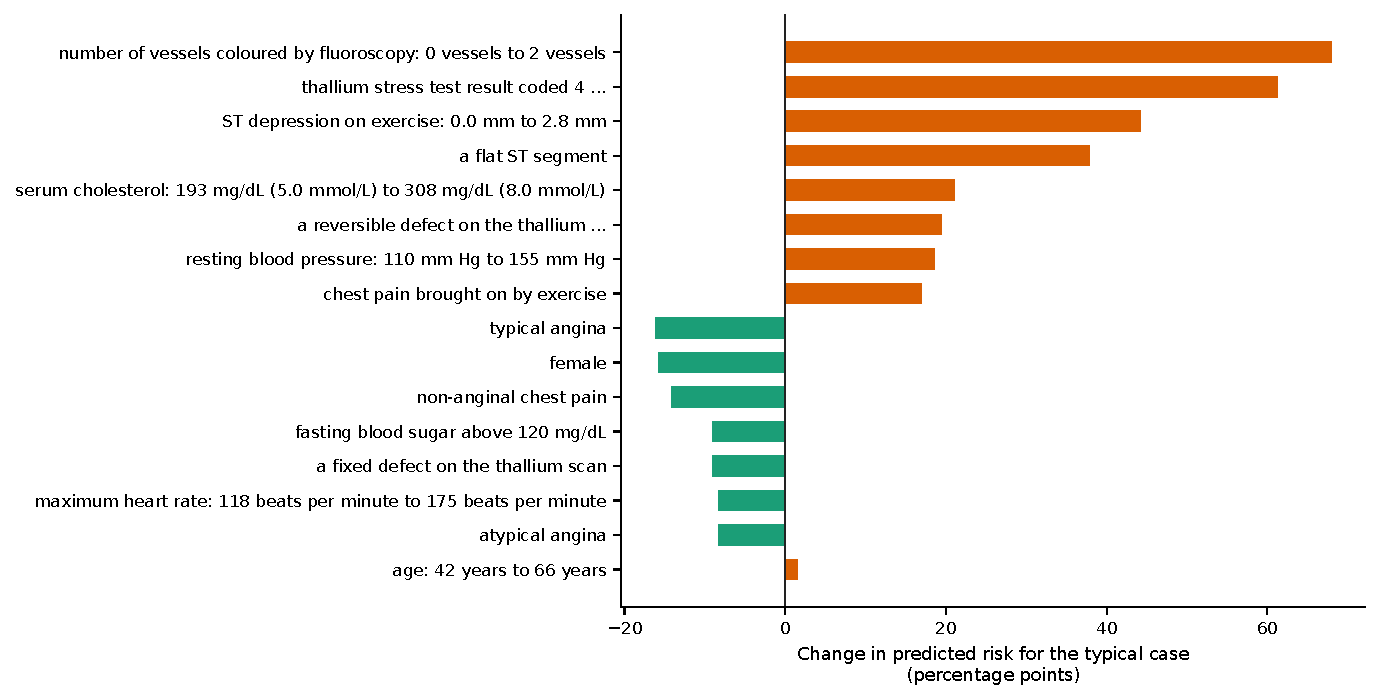
\includegraphics[width=\linewidth,height=0.88\textheight,keepaspectratio]{figures/heart-s5-c3/ann_29-effects.pdf}
\caption{The whole model: Each input's change in the predicted value for the typical case across the whole model, largest first (orange: raises it, teal: lowers it).}
\label{fig:hearts5c3:plot-ann29-0}
\end{figure}
\par\smallskip\noindent{\small \textbf{Dive deeper:} ST depression signal (\ref{rd:ann27}); Age term (\ref{rd:ann28}). Technical detail: \ref{tech:ann29}.\par}
\subsubsection{ST depression signal}\label{rd:ann27}
\noindent{\footnotesize Part of: The whole model (\ref{rd:ann29}).\par}
\noindent{\small Figure~\ref{fig:hearts5c3:parts-ann27} shows what feeds this part; Figure~\ref{fig:hearts5c3:units-ann27} its units and every connection into them (dashed boxes: connections from or to other parts, drawn in their own sections).\par}
\begin{figure}[H]\centering
\resizebox{!}{\ifdim\height>0.5\textheight 0.5\textheight\else\height\fi}{%
\resizebox{\ifdim\width>\linewidth\linewidth\else\width\fi}{!}{%
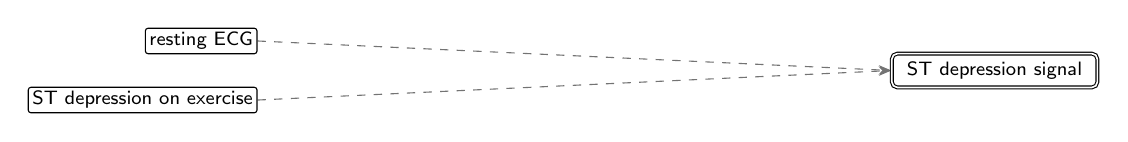
\begin{tikzpicture}[
  font=\sffamily\scriptsize, >={Stealth[length=1.6mm]},
  inp/.style={draw, rounded corners=1pt, fill=white, inner sep=1.5pt, minimum height=3.2mm, anchor=east},
  abox/.style={draw, thick, rounded corners=2pt, align=center, inner sep=3pt, minimum height=6mm, text width=42mm},
  outp/.style={draw, double, rounded corners=2pt, fill=white, align=center, inner sep=3pt, text width=24mm},
  agg/.style={draw=black!55},
]
\node[inp] (i0) at (0,0.375) {resting ECG};
\node[inp] (i1) at (0,-0.375) {ST depression on exercise};
\node[outp] (out) at (9.36,0) {ST depression signal};
\begin{scope}[on background layer]
\draw[->, agg, thin, dashed] (i0.east) -- (out.west);
\draw[->, agg, thin, dashed] (i1.east) -- (out.west);
\end{scope}
\end{tikzpicture}}}%
\caption{ST depression signal: what feeds it, one level down.}
\label{fig:hearts5c3:parts-ann27}
\end{figure}
\begin{figure}[H]\centering
\resizebox{\ifdim\width>\linewidth\linewidth\else\width\fi}{!}{%
\definecolor{netup}{HTML}{D95F02}\definecolor{netdown}{HTML}{1B9E77}\definecolor{netmixed}{HTML}{7F7F7F}%
\begin{tikzpicture}[
  font=\sffamily\scriptsize, >={Stealth[length=1.4mm]},
  inp/.style={draw, circle, fill=white, minimum size=3.2mm, inner sep=0pt},
  hid/.style={draw, circle, fill=white, minimum size=5.2mm, inner sep=0.5pt, font=\sffamily\tiny},
  exitbox/.style={draw, thick, rectangle, fill=white, align=center, text width=17mm, minimum height=5mm, inner sep=1.5pt, font=\sffamily\tiny},
  sumbox/.style={draw, thick, dashed, rectangle, fill=white, align=center, text width=17mm, minimum height=5mm, inner sep=1.5pt, font=\sffamily\tiny},
  outp/.style={draw, thick, regular polygon, regular polygon sides=6, fill=white, minimum size=10mm, inner sep=0pt, font=\sffamily\tiny, align=center},
  stub/.style={draw, dashed, rounded corners=2pt, fill=white, align=center, inner sep=2pt, font=\sffamily\tiny, text width=15mm},
  inlab/.style={font=\sffamily\tiny, align=center, text width=15mm, inner sep=1pt, fill=white, fill opacity=0.8, text opacity=1},
  wpos/.style={draw=NavyBlue}, wneg/.style={draw=BrickRed}, wagg/.style={draw=black!45, line width=1.2pt},
  wmix/.style={draw=Plum},
]
\node[hid] (n290) at (2.0,4.6) {h2};
\node[hid] (n204) at (2.0,1.9) {h1};
\node[hid] (n3487) at (2.0,3.25) {h4};
\node[inp, draw=netup, very thick] (ninxxoldpeak) at (1.1,0.0) {};
\path (ninxxoldpeak.south) node[inlab, anchor=north] (labninxxoldpeak) {ST depression $\uparrow$};
\node[inp, draw=netup, very thick] (ninxxrestecgx0) at (2.9,0.0) {};
\path (ninxxrestecgx0.south) node[inlab, anchor=north] (labninxxrestecgx0) {normal ECG $\uparrow$};
\node[stub] (ntoxxthexmodelxoutput) at (2.0,6.15) {to the model output};
\begin{scope}[on background layer]
\node[fit=(n290) (n204) (n3487) , inner sep=8pt, rounded corners=5pt, fill=BurntOrange!10, draw=BurntOrange!45] (clu0) {};
\draw[->, wpos, line width=1.13pt] (ninxxoldpeak) -- (n204);
\draw[->, wpos, line width=0.60pt] (n204) -- (n290);
\draw[->, wpos, line width=0.58pt] (n204) -- (n3487);
\draw[->, wpos, line width=0.55pt] (n3487) -- (n290);
\draw[->, wpos, line width=0.59pt] (ninxxrestecgx0) -- (n204);
\draw[->, wpos, line width=0.27pt] (n204) -- (ntoxxthexmodelxoutput);
\draw[->, wpos, line width=0.33pt] (n290) -- (ntoxxthexmodelxoutput);
\end{scope}
\node[font=\sffamily\scriptsize\bfseries, text=BurntOrange!55!black, anchor=south west, inner sep=1pt, fill=white, fill opacity=0.85, text opacity=1] at (clu0.north west) {ST depression signal};
\end{tikzpicture}}%
\caption{ST depression signal: its units and every connection into them. Blue: positive weight (raises the score); red: negative weight (lowers it); thicker: larger weight. Orange outline and up arrow: raises the final prediction; teal and down arrow: lowers it; grey and double arrow: depends.}
\label{fig:hearts5c3:units-ann27}
\end{figure}
\paragraph{Hypothesis.} This part raises the predicted risk with ST depression on exercise, adding nothing until about 0.5 mm and then steadily, and more so with a normal resting ECG.\,{\scriptsize\textcolor{NavyBlue}{[C26, C28]}}
\paragraph{Evidence.} It acts on 105 of 242 training patients, 66 of whom had heart disease; for the typical patient it acts on, the predicted risk is about 76\% without it and about 91\% with it.\,{\scriptsize\textcolor{NavyBlue}{[C30]}} Through it, more ST depression adds nothing until about 0.5 mm, then raises the predicted risk steadily: for a typical patient from about 16\% at 0 mm to about 60\% at 2.8 mm.\,{\scriptsize\textcolor{NavyBlue}{[C26]}} ST depression counts more with a normal resting ECG, nothing until about 0.5 mm and then steadily, from about 16\% to about 60\%, against about 21\% to about 48\% with any other resting ECG.\,{\scriptsize\textcolor{NavyBlue}{[C28]}} Through it, a resting ECG other than normal lowers a typical patient's risk from about 18\% to about 16\%.\,{\scriptsize\textcolor{NavyBlue}{[C27]}} Its formula reproduces the part exactly on all 242 training patients.\,{\scriptsize\textcolor{NavyBlue}{[C31]}}
\par\noindent{\small Evidence plots: Figure~\ref{fig:hearts5c3:plot-ann27-0}, Figure~\ref{fig:hearts5c3:plot-ann27-1}, Figure~\ref{fig:hearts5c3:plot-ann27-2}, Figure~\ref{fig:hearts5c3:plot-ann27-3}, Figure~\ref{fig:hearts5c3:plot-ann27-4}, Figure~\ref{fig:hearts5c3:plot-ann27-5}.\par}
\par\noindent{\small Figure~\ref{fig:hearts5c3:plot-ann27-3} shows this part's own output, unit h1: it switches on at about 0.4548 mm of ST depression on exercise, and is zero below.\par}
\par\noindent{\small Figure~\ref{fig:hearts5c3:plot-ann27-4} shows this part's own output, unit h2: it switches on at about 0.5774 mm of ST depression on exercise, and is zero below.\par}
\begin{figure}[H]\centering
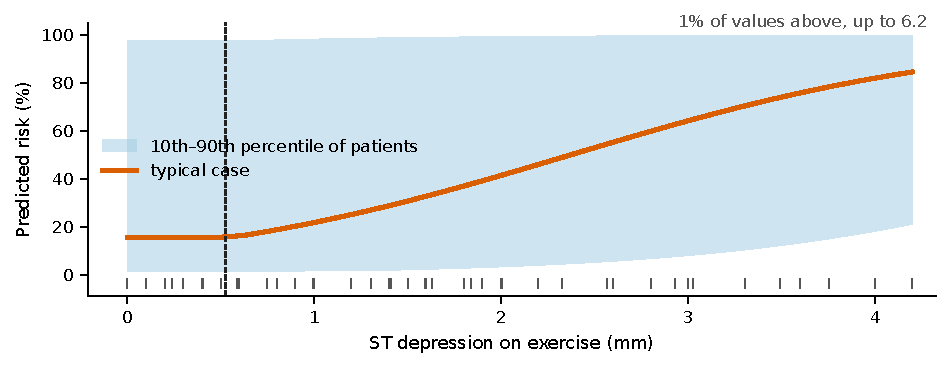
\includegraphics[width=\linewidth,height=0.88\textheight,keepaspectratio]{figures/heart-s5-c3/ann_27-response.pdf}
\caption{ST depression signal: Response curves through this part: the typical case (bold), the 10th to 90th percentile of individual patients (band), the fold or step point (dashed) with its spread across them (grey), and the observed values (ticks).}
\label{fig:hearts5c3:plot-ann27-0}
\end{figure}
\begin{figure}[H]\centering
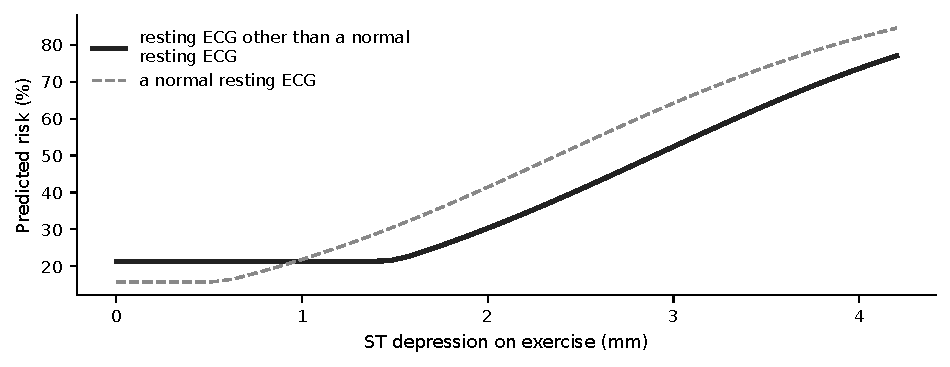
\includegraphics[width=\linewidth,height=0.88\textheight,keepaspectratio]{figures/heart-s5-c3/ann_27-interaction.pdf}
\caption{ST depression signal: How the effect differs between groups: one curve per group, for the typical case of each group.}
\label{fig:hearts5c3:plot-ann27-1}
\end{figure}
\begin{figure}[H]\centering
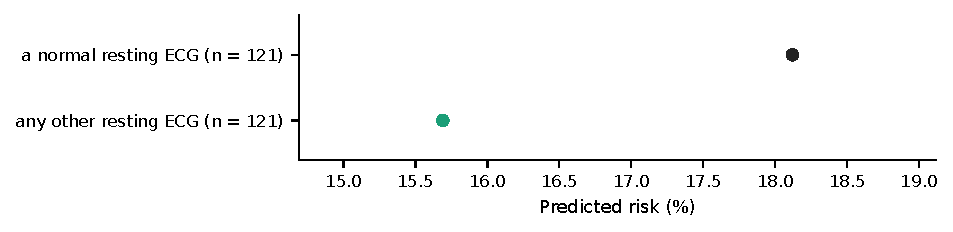
\includegraphics[width=\linewidth,height=0.88\textheight,keepaspectratio]{figures/heart-s5-c3/ann_27-categories-small.pdf}
\caption{ST depression signal: The predicted value for the typical case at each level, through this part (n = training patients; grey: fewer than 20).}
\label{fig:hearts5c3:plot-ann27-2}
\end{figure}
\begin{figure}[H]\centering
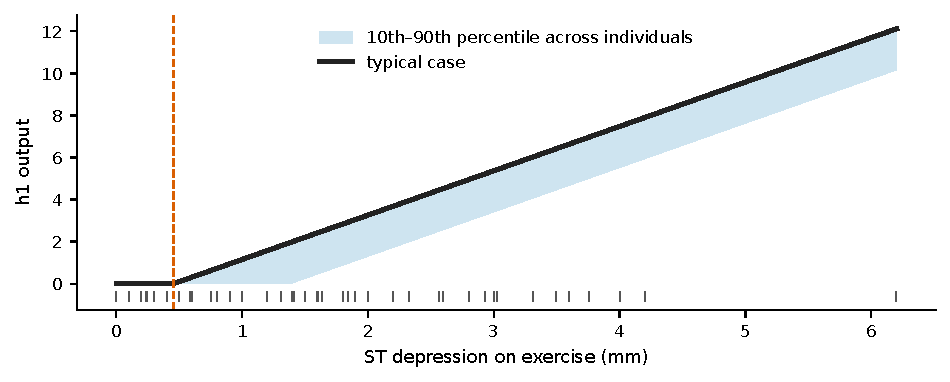
\includegraphics[width=\linewidth,height=0.88\textheight,keepaspectratio]{figures/heart-s5-c3/ann_27-partial-204.pdf}
\caption{ST depression signal: This part's own output, unit h1 (the output of 'ST depression signal'), on its own scale (its activation), with every other input at the typical case; it is active for 105 of 242. Bold: the typical case; band: 10th to 90th percentile across individuals; dashed: where it switches on; ticks: the data.}
\label{fig:hearts5c3:plot-ann27-3}
\end{figure}
\begin{figure}[H]\centering
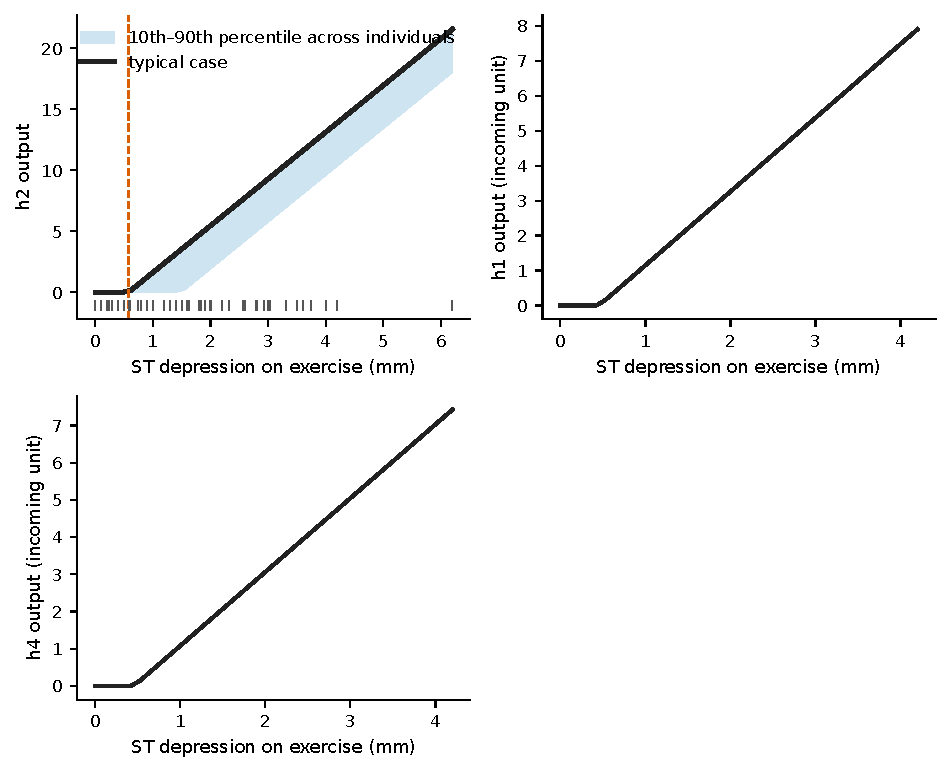
\includegraphics[width=\linewidth,height=0.88\textheight,keepaspectratio]{figures/heart-s5-c3/ann_27-partial-290.pdf}
\caption{ST depression signal: This part's own output, unit h2 (combines 2 non-linear units), on its own scale (its activation), with every other input at the typical case; it is active for 96 of 242. Bold: the typical case; band: 10th to 90th percentile across individuals; dashed: where it switches on; ticks: the data.}
\label{fig:hearts5c3:plot-ann27-4}
\end{figure}
\begin{figure}[H]\centering
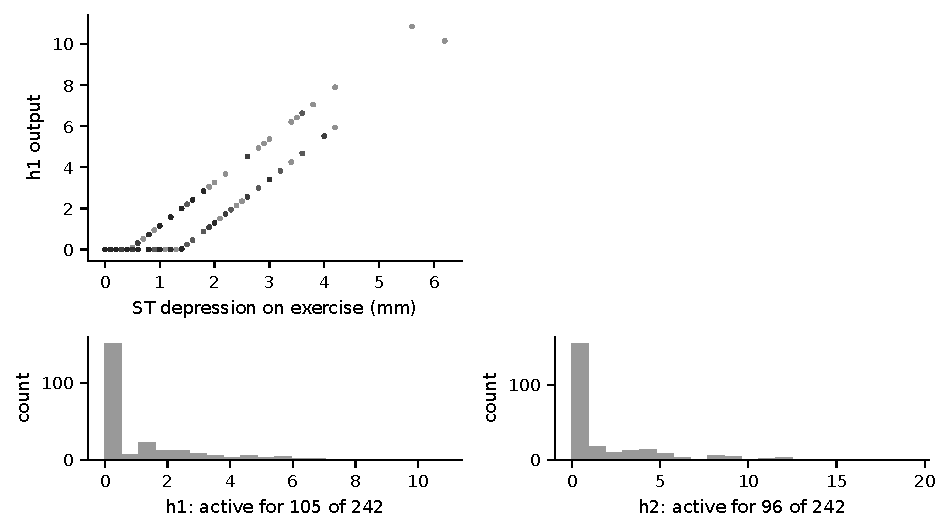
\includegraphics[width=\linewidth,height=0.88\textheight,keepaspectratio]{figures/heart-s5-c3/ann_27-units.pdf}
\caption{ST depression signal: This part's hidden units: each unit's output against its main numeric input (top) and how often it is active (bottom).}
\label{fig:hearts5c3:plot-ann27-5}
\end{figure}
\par\smallskip\noindent{\small Technical detail: \ref{tech:ann27}.\par}
\subsubsection{Age term}\label{rd:ann28}
\noindent{\footnotesize Part of: The whole model (\ref{rd:ann29}).\par}
\noindent{\small Figure~\ref{fig:hearts5c3:parts-ann28} shows what feeds this part; Figure~\ref{fig:hearts5c3:units-ann28} its units and every connection into them (dashed boxes: connections from or to other parts, drawn in their own sections).\par}
\begin{figure}[H]\centering
\resizebox{!}{\ifdim\height>0.5\textheight 0.5\textheight\else\height\fi}{%
\resizebox{\ifdim\width>\linewidth\linewidth\else\width\fi}{!}{%
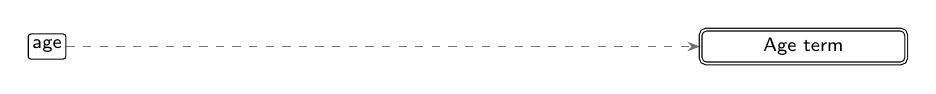
\begin{tikzpicture}[
  font=\sffamily\scriptsize, >={Stealth[length=1.6mm]},
  inp/.style={draw, rounded corners=1pt, fill=white, inner sep=1.5pt, minimum height=3.2mm, anchor=east},
  abox/.style={draw, thick, rounded corners=2pt, align=center, inner sep=3pt, minimum height=6mm, text width=42mm},
  outp/.style={draw, double, rounded corners=2pt, fill=white, align=center, inner sep=3pt, text width=24mm},
  agg/.style={draw=black!55},
]
\node[inp] (i0) at (0,-0.0) {age};
\node[outp] (out) at (9.36,0) {Age term};
\begin{scope}[on background layer]
\draw[->, agg, thin, dashed] (i0.east) -- (out.west);
\end{scope}
\end{tikzpicture}}}%
\caption{Age term: what feeds it, one level down.}
\label{fig:hearts5c3:parts-ann28}
\end{figure}
\begin{figure}[H]\centering
\resizebox{\ifdim\width>\linewidth\linewidth\else\width\fi}{!}{%
\definecolor{netup}{HTML}{D95F02}\definecolor{netdown}{HTML}{1B9E77}\definecolor{netmixed}{HTML}{7F7F7F}%
\begin{tikzpicture}[
  font=\sffamily\scriptsize, >={Stealth[length=1.4mm]},
  inp/.style={draw, circle, fill=white, minimum size=3.2mm, inner sep=0pt},
  hid/.style={draw, circle, fill=white, minimum size=5.2mm, inner sep=0.5pt, font=\sffamily\tiny},
  exitbox/.style={draw, thick, rectangle, fill=white, align=center, text width=17mm, minimum height=5mm, inner sep=1.5pt, font=\sffamily\tiny},
  sumbox/.style={draw, thick, dashed, rectangle, fill=white, align=center, text width=17mm, minimum height=5mm, inner sep=1.5pt, font=\sffamily\tiny},
  outp/.style={draw, thick, regular polygon, regular polygon sides=6, fill=white, minimum size=10mm, inner sep=0pt, font=\sffamily\tiny, align=center},
  stub/.style={draw, dashed, rounded corners=2pt, fill=white, align=center, inner sep=2pt, font=\sffamily\tiny, text width=15mm},
  inlab/.style={font=\sffamily\tiny, align=center, text width=15mm, inner sep=1pt, fill=white, fill opacity=0.8, text opacity=1},
  wpos/.style={draw=NavyBlue}, wneg/.style={draw=BrickRed}, wagg/.style={draw=black!45, line width=1.2pt},
  wmix/.style={draw=Plum},
]
\node[exitbox] (n1987) at (1.0,1.9) {Age term $\uparrow$};
\node[inp, draw=netup, very thick] (ninxxage) at (1.0,0.0) {};
\path (ninxxage.south) node[inlab, anchor=north] (labninxxage) {age $\uparrow$};
\node[stub] (ntoxxthexmodelxoutput) at (1.0,3.45) {to the model output};
\begin{scope}[on background layer]
\node[fit=(n1987) , inner sep=8pt, rounded corners=5pt, fill=ForestGreen!10, draw=ForestGreen!45] (clu0) {};
\draw[->, wpos, line width=0.56pt] (ninxxage) -- (n1987);
\draw[->, wpos, line width=0.28pt] (n1987) -- (ntoxxthexmodelxoutput);
\end{scope}
\node[font=\sffamily\scriptsize\bfseries, text=ForestGreen!55!black, anchor=south west, inner sep=1pt, fill=white, fill opacity=0.85, text opacity=1] at (clu0.north west) {Age term};
\end{tikzpicture}}%
\caption{Age term: its units and every connection into them. Blue: positive weight (raises the score); red: negative weight (lowers it); thicker: larger weight. Orange outline and up arrow: raises the final prediction; teal and down arrow: lowers it; grey and double arrow: depends.}
\label{fig:hearts5c3:units-ann28}
\end{figure}
\paragraph{Hypothesis.} This part adds a little to the predicted risk for older patients: nothing until about 53 years, then steadily.\,{\scriptsize\textcolor{NavyBlue}{[C32, C33]}}
\paragraph{Evidence.} It acts on 148 of 242 training patients, 81 of whom had heart disease; for the typical patient it acts on, the predicted risk is about 91\% without it and about 92\% with it.\,{\scriptsize\textcolor{NavyBlue}{[C34]}} Through it, age adds nothing until about 53 years, then raises the risk steadily, for a typical patient from about 18\% at 42 to about 19\% at 66 years.\,{\scriptsize\textcolor{NavyBlue}{[C32, C33]}} Its formula reproduces the part exactly on all 242 training patients.\,{\scriptsize\textcolor{NavyBlue}{[C36]}}
\par\noindent{\small Evidence plots: Figure~\ref{fig:hearts5c3:plot-ann28-0}, Figure~\ref{fig:hearts5c3:plot-ann28-1}, Figure~\ref{fig:hearts5c3:plot-ann28-2}.\par}
\par\noindent{\small Figure~\ref{fig:hearts5c3:plot-ann28-1} shows this part's own output, unit h3: it switches on at about 52.81 years of age, and is zero below.\par}
\begin{figure}[H]\centering
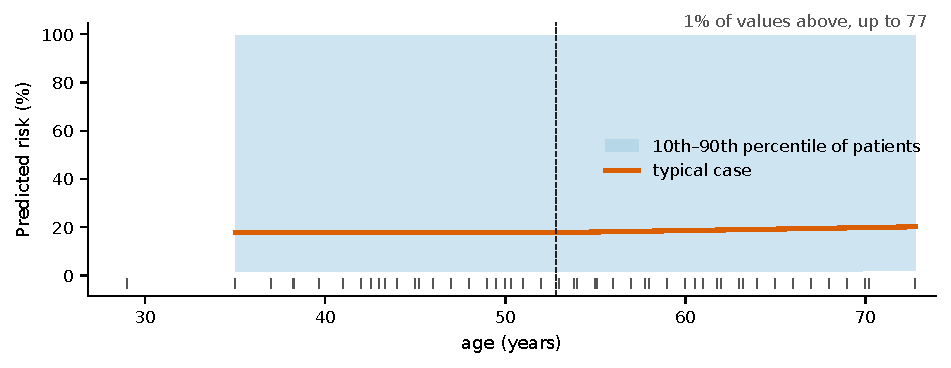
\includegraphics[width=\linewidth,height=0.88\textheight,keepaspectratio]{figures/heart-s5-c3/ann_28-response.pdf}
\caption{Age term: Response curves through this part: the typical case (bold), the 10th to 90th percentile of individual patients (band), the fold or step point (dashed) with its spread across them (grey), and the observed values (ticks).}
\label{fig:hearts5c3:plot-ann28-0}
\end{figure}
\begin{figure}[H]\centering
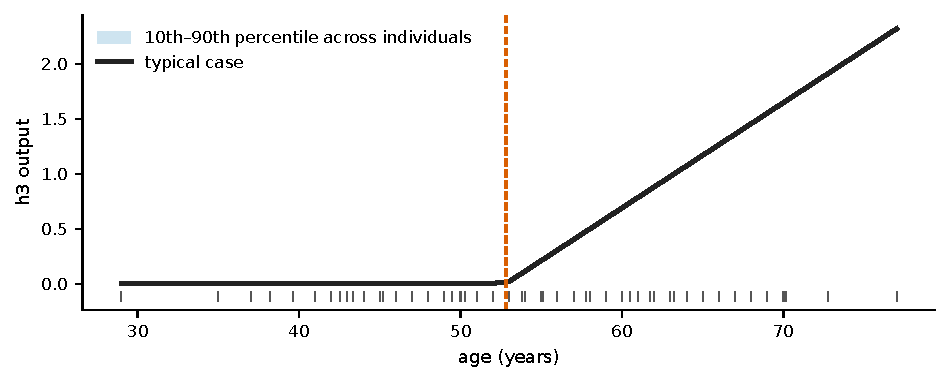
\includegraphics[width=\linewidth,height=0.88\textheight,keepaspectratio]{figures/heart-s5-c3/ann_28-partial-1987.pdf}
\caption{Age term: This part's own output, unit h3 (the output of 'Age term'), on its own scale (its activation), with every other input at the typical case; it is active for 148 of 242. Bold: the typical case; band: 10th to 90th percentile across individuals; dashed: where it switches on; ticks: the data.}
\label{fig:hearts5c3:plot-ann28-1}
\end{figure}
\begin{figure}[H]\centering
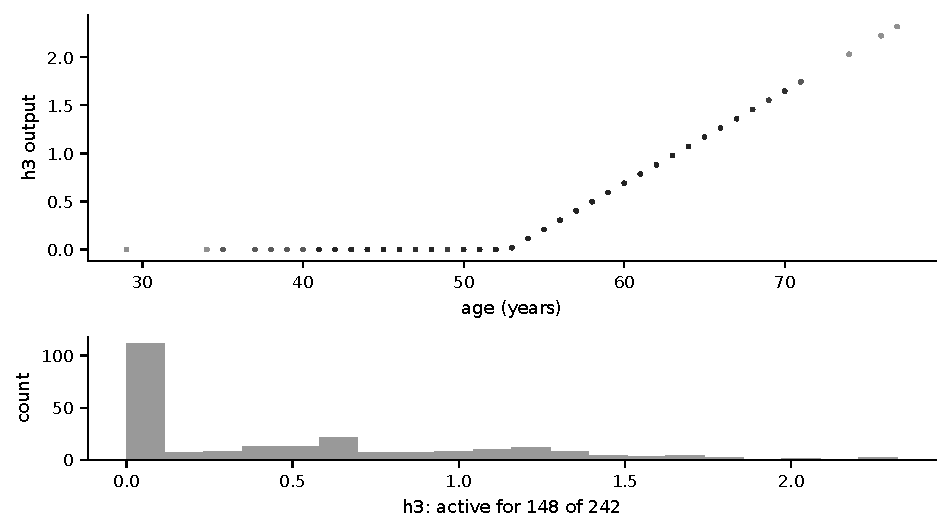
\includegraphics[width=\linewidth,height=0.88\textheight,keepaspectratio]{figures/heart-s5-c3/ann_28-units.pdf}
\caption{Age term: This part's hidden units: each unit's output against its main numeric input (top) and how often it is active (bottom).}
\label{fig:hearts5c3:plot-ann28-2}
\end{figure}
\par\smallskip\noindent{\small Technical detail: \ref{tech:ann28}.\par}
\subsection{Not supported by the model}
\begin{itemize}\setlength\itemsep{0pt}\small
\item C17: direction claim about resting ECG in the whole model: not supported by the model (44\% of patients have the opposite sign (allowed: 10\%)).
\item C29: threshold claim about ST depression during exercise (compared with rest) in part ann\_\allowbreak{}27: not supported by the model (the fold changes the curve by only 0.095 log-odds compared with a straight line (needed 0.1)).
\item C35: null claim about age in part ann\_\allowbreak{}28: not supported by the model (predictions move by up to 0.032).
\end{itemize}
\clearpage\section*{Technical detail: heart-s5-c3}
\addcontentsline{toc}{section}{Technical detail: heart-s5-c3}
\noindent{\small The record behind each part: the original hypothesis, the closed form, and every claim with its estimate (log-odds and odds ratio), range across patients, n and test check.\par}
\renewcommand{\thesubsection}{T.\arabic{subsection}}\setcounter{subsection}{0}
\subsection{The whole model}\label{tech:ann29}
\noindent{\footnotesize Annotation ann\_\allowbreak{}29 (heart\_\allowbreak{}disease\_\allowbreak{}logit). Reads: age, sex, chest pain type, resting blood pressure, serum cholesterol, fasting blood sugar, resting ECG, maximum heart rate reached during the exercise test, exercise-induced angina, ST depression during exercise (compared with rest), slope of the ST segment at peak exercise, number of major vessels coloured by fluoroscopy, thallium stress test result.\par}
\paragraph{Original hypothesis (unchanged).} Root: p = sigmoid(z), z = -0.536 + LINEAR CORE + 0.049*\allowbreak{}ischaemia\_\allowbreak{}chain[204]\allowbreak{} + 0.216*\allowbreak{}ischaemia\_\allowbreak{}chain[290]\allowbreak{} + 0.082*age\_\allowbreak{}hinge. LINEAR CORE (17 direct input-$>$output edges, z-scored inputs): ca +1.485, sex:0 -1.042, slope:1 -0.873, chol +0.551, cp:1 -0.494, trestbps +0.483, thal:3 -0.471, cp:3 -0.442, slope:3 -0.434, exang:1 +0.423, thal:6 -0.421, cp:4 +0.354, fbs:0 +0.274, thalach -0.213, restecg:0 -0.188, thal:4 +0.172, thal:7 +0.025. Seven inputs are unconnected (sex:1, cp:2, fbs:1, restecg:1, restecg:2, exang:0, slope:2; zero-effect entries of this root). Oldpeak and age have no direct edge and act only through the children; restecg:0 acts both directly and through the ischaemia chain (split into restecg:0\_\allowbreak{}a direct and restecg:0\_\allowbreak{}b). COMPOSITION: additive. The two children are read out additively into z: ischaemia\_\allowbreak{}chain (two exits: a one-sided ST-depression score opened earlier by a normal resting ECG, and a steeper second stage of the same score) and age\_\allowbreak{}hinge (an age term that starts just below the median age). Together the chain gives oldpeak a hinge-shaped effect: about 0.12 logit per SD between its two thresholds and about 1.10 per SD above the second (z-oldpeak -0.39 with a normal ECG, +0.40 otherwise). EVIDENCE (train, n=242): full model AUC 0.9376, acc 0.888 (compute\_\allowbreak{}performance)\allowbreak{}. Linear core alone AUC 0.9317; logit SD 3.22 (core) vs 0.80 (nonlinear readouts). Removing the whole chain (204 with downstream) gives 0.9317; readout-only ablations: 204 0.9380, 290 0.9341, age 0.9371. All ReLUs as identities 0.9304; one least-squares linear fit of all nonlinear readouts on restecg:0, oldpeak and age gives 0.9355 (R2 0.88); an L2 logistic regression on all 26 inputs gives 0.9355. Mean $|$SHAP$|$ (kernel, all 242 train rows): ca 0.141, sex:0 0.104, slope:1 0.099, oldpeak 0.060, thal:3 0.054, exang:1 0.045, chol 0.044, cp:3 0.043, cp:4 0.040, trestbps 0.040. Interpretation: close to logistic regression plus one ST-depression correction that switches on above a threshold (lower for patients with a normal resting ECG) and a small age term above median age. Counter-directional signs reported, not explained: a normal resting ECG lowers the oldpeak threshold inside the chain (raising risk), fbs:0 (normal fasting sugar) +0.27 directly, thal:7 (reversible defect) only +0.025. Compared with the 10-seed heart-s5 record (generation 37, key 9330: ischaemia gate -$>$ resting-BP gate -$>$ age term) and its cluster-1 sibling: the same ischaemia gate on oldpeak and restecg:0, but here the second stage is a steeper copy of the score (no resting-BP offset) and the age term is a free-standing hinge (not switched off by the chain).
\paragraph{Closed form.} Read through its parts (their formulas are in their own sections).
\paragraph{Split inputs.} To annotate the parts, the explanation split these inputs into copies (a refactoring step that does not change what the model computes); the diagrams draw each input once: normal ECG (2 copies).
\paragraph{Evidence table} (next page, landscape).
\begin{landscape}
{\scriptsize\setlength{\tabcolsep}{3pt}\renewcommand{\arraystretch}{1.15}
\rowcolors{2}{black!6}{white}
\begin{longtable}{@{}l>{\raggedright\arraybackslash}p{0.36\linewidth}>{\raggedright\arraybackslash}p{0.14\linewidth}rrr>{\raggedright\arraybackslash}p{0.06\linewidth}>{\raggedright\arraybackslash}p{0.17\linewidth}c@{}}
\toprule\rowcolor{white}
ID & What is checked & Risk, typical patient & Log-odds & OR & Range (p10--p90) & n & Test check & OK \\
\midrule\endfirsthead
\toprule\rowcolor{white}
ID & What is checked & Risk, typical patient & Log-odds & OR & Range (p10--p90) & n & Test check & OK \\
\midrule\endhead
\bottomrule\endfoot
C01 & direction: number of vessels coloured by fluoroscopy: 0 vessels to 2 vessels (whole model) \newline{\itshape shape: steady (equal steps); 100\% of patients same; verified; risk saturates near 100\%} & 18\% to 86\% & 3.33 & 28.0 & 3.33 to 3.33 & 242 & unclear; AUC gain 0.029 [-0.039, 0.100] & \textcolor{OliveGreen}{yes} \\
C02 & direction: thallium stress test result: a normal thallium scan to thallium stress test result coded 4 (meaning not recorded) (whole model) \newline{\itshape shape: categorical; highest to lowest: thallium stress test result coded 4 (meaning not recorded), a reversible defect on the thallium scan, a normal thallium scan, a fixed defect on the thallium scan} & 18\% to 79\% & 2.85 & 17.4 & 2.85 to 2.85 & 135, 2 (small n) & unclear; AUC gain 0.020 [-0.012, 0.058] & \textcolor{OliveGreen}{yes} \\
C03 & direction: ST depression on exercise: 0.0 mm to 2.8 mm (whole model) \newline{\itshape shape: hinge at 0.5 mm; 100\% of patients same; verified} & 16\% to 60\% & 1.65 & 5.20 & 1.22 to 2.08 & 242 & unclear; AUC gain 0.023 [-0.001, 0.055] & \textcolor{OliveGreen}{yes} \\
C04 & direction: slope of the ST segment at peak exercise: an upsloping ST segment to a flat ST segment (whole model) \newline{\itshape shape: categorical; highest to lowest: a flat ST segment, a downsloping ST segment, an upsloping ST segment} & 18\% to 56\% & 1.75 & 5.75 & 1.75 to 1.75 & 115, 110 & disagrees; AUC gain -0.024 [-0.071, 0.009] & \textcolor{OliveGreen}{yes} \\
C05 & direction: serum cholesterol: 193 mg/dL (5.0 mmol/L) to 308 mg/dL (8.0 mmol/L) (whole model) \newline{\itshape shape: steady; 100\% of patients same; verified} & 11\% to 33\% & 1.32 & 3.73 & 1.32 to 1.32 & 242 & disagrees; AUC gain -0.019 [-0.058, 0.008] & \textcolor{OliveGreen}{yes} \\
C06 & direction: thallium stress test result: a normal thallium scan to a reversible defect on the thallium scan (whole model) \newline{\itshape shape: categorical; highest to lowest: thallium stress test result coded 4 (meaning not recorded), a reversible defect on the thallium scan, a normal thallium scan, a fixed defect on the thallium scan} & 18\% to 38\% & 1.00 & 2.72 & 1.00 to 1.00 & 135, 90 & unclear; AUC gain 0.020 [-0.012, 0.058] & \textcolor{OliveGreen}{yes} \\
C07 & direction: resting blood pressure: 110 mm Hg to 155 mm Hg (whole model) \newline{\itshape shape: steady; 100\% of patients same; verified} & 12\% to 30\% & 1.19 & 3.30 & 1.19 to 1.19 & 242 & unclear; AUC gain 0.008 [-0.018, 0.037] & \textcolor{OliveGreen}{yes} \\
C08 & direction: exercise-induced angina: no chest pain on exercise to chest pain brought on by exercise (whole model) \newline{\itshape shape: categorical; highest to lowest: chest pain brought on by exercise, no chest pain on exercise} & 18\% to 35\% & 0.89 & 2.44 & 0.89 to 0.89 & 160, 82 & agrees; AUC gain 0.022 [0.003, 0.049] & \textcolor{OliveGreen}{yes} \\
C09 & direction: chest pain type: no chest pain (asymptomatic) to typical angina (whole model) \newline{\itshape shape: categorical; highest to lowest: no chest pain (asymptomatic), atypical angina, non-anginal chest pain, typical angina} & 18\% to 2\% & -2.43 & 0.09 & -2.43 to -2.43 & 108, 22 & agrees; AUC gain 0.033 [0.008, 0.066] & \textcolor{OliveGreen}{yes} \\
C10 & direction: sex: male to female (whole model) \newline{\itshape shape: categorical; highest to lowest: male, female} & 18\% to 2\% & -2.19 & 0.11 & -2.19 to -2.19 & 159, 83 & unclear; AUC gain 0.025 [-0.007, 0.066] & \textcolor{OliveGreen}{yes} \\
C11 & direction: chest pain type: no chest pain (asymptomatic) to non-anginal chest pain (whole model) \newline{\itshape shape: categorical; highest to lowest: no chest pain (asymptomatic), atypical angina, non-anginal chest pain, typical angina} & 18\% to 4\% & -1.69 & 0.18 & -1.69 to -1.69 & 108, 70 & agrees; AUC gain 0.033 [0.008, 0.066] & \textcolor{OliveGreen}{yes} \\
C12 & direction: fasting blood sugar: fasting blood sugar of 120 mg/dL or less to fasting blood sugar above 120 mg/dL (whole model) \newline{\itshape shape: categorical; highest to lowest: fasting blood sugar of 120 mg/dL or less, fasting blood sugar above 120 mg/dL} & 18\% to 9\% & -0.80 & 0.45 & -0.80 to -0.80 & 209, 33 & unclear; AUC gain 0.000 [-0.013, 0.013] & \textcolor{OliveGreen}{yes} \\
C13 & direction: thallium stress test result: a normal thallium scan to a fixed defect on the thallium scan (whole model) \newline{\itshape shape: categorical; highest to lowest: thallium stress test result coded 4 (meaning not recorded), a reversible defect on the thallium scan, a normal thallium scan, a fixed defect on the thallium scan} & 18\% to 9\% & -0.80 & 0.45 & -0.80 to -0.80 & 135, 15 (small n) & unclear; AUC gain 0.020 [-0.012, 0.058] & \textcolor{OliveGreen}{yes} \\
C14 & direction: maximum heart rate: 118 beats per minute to 175 beats per minute (whole model) \newline{\itshape shape: steady; 100\% of patients same; verified} & 23\% to 15\% & -0.54 & 0.58 & -0.54 to -0.54 & 242 & agrees; AUC gain 0.014 [0.002, 0.035] & \textcolor{OliveGreen}{yes} \\
C15 & direction: chest pain type: no chest pain (asymptomatic) to atypical angina (whole model) \newline{\itshape shape: categorical; highest to lowest: no chest pain (asymptomatic), atypical angina, non-anginal chest pain, typical angina} & 18\% to 10\% & -0.71 & 0.49 & -0.71 to -0.71 & 108, 42 & agrees; AUC gain 0.033 [0.008, 0.066] & \textcolor{OliveGreen}{yes} \\
C16 & direction: resting ECG: a normal resting ECG to resting ECG other than a normal resting ECG (direct contribution only, not through any part) \newline{\itshape shape: categorical; highest to lowest: resting ECG other than a normal resting ECG, a normal resting ECG} & 18\% to 24\% & 0.38 & 1.46 & 0.38 to 0.38 & 121, 121 & unclear; AUC gain 0.005 [-0.005, 0.024] & \textcolor{OliveGreen}{yes} \\
C17 & direction: resting ECG: a normal resting ECG to resting ECG other than a normal resting ECG (whole model) \newline{\itshape shape: categorical; highest to lowest: resting ECG other than a normal resting ECG, a normal resting ECG} & 18\% to 21\% & 0.02 & 1.02 & -0.49 to 0.38 & 121, 121 & disagrees; AUC gain 0.003 [-0.013, 0.021] & \textcolor{BrickRed}{no} \\
C18 & direction: age: 42 years to 66 years (whole model) \newline{\itshape shape: hinge at 53 years; 100\% of patients same; verified; matches the fold at 53 years} & 18\% to 19\% & 0.10 & 1.11 & 0.10 to 0.10 & 242 & disagrees; AUC gain -0.003 [-0.017, 0.004] & \textcolor{OliveGreen}{yes} \\
C19 & direction: slope of the ST segment at peak exercise: an upsloping ST segment to a downsloping ST segment (whole model) \newline{\itshape shape: categorical; highest to lowest: a flat ST segment, a downsloping ST segment, an upsloping ST segment} & 18\% to 19\% & 0.05 & 1.05 & 0.05 to 0.05 & 115, 17 (small n) & disagrees; AUC gain -0.024 [-0.071, 0.009] & \textcolor{OliveGreen}{yes} \\
C20 & magnitude: number of vessels coloured by fluoroscopy: 0 vessels to 2 vessels, typical patient \newline{\itshape shape: steady (equal steps); 100\% of patients same; verified; risk saturates near 100\%} & 18\% to 86\% & 3.33 & 28.0 &  & 242 & unclear; AUC gain 0.029 [-0.039, 0.100] & \textcolor{OliveGreen}{yes} \\
C21 & magnitude: ST depression on exercise: 0.0 mm to 2.8 mm, typical patient \newline{\itshape shape: hinge at 0.5 mm; 100\% of patients same; verified} & 16\% to 60\% & 2.08 & 8.01 &  & 242 & unclear; AUC gain 0.023 [-0.001, 0.055] & \textcolor{OliveGreen}{yes} \\
C22 & magnitude: slope of the ST segment at peak exercise: an upsloping ST segment to a flat ST segment, typical patient \newline{\itshape shape: categorical; highest to lowest: a flat ST segment, a downsloping ST segment, an upsloping ST segment} & 18\% to 56\% & 1.75 & 5.75 &  & 115, 110 & disagrees; AUC gain -0.024 [-0.071, 0.009] & \textcolor{OliveGreen}{yes} \\
C23 & magnitude: serum cholesterol: 193 mg/dL (5.0 mmol/L) to 308 mg/dL (8.0 mmol/L), typical patient \newline{\itshape shape: steady; 100\% of patients same; verified} & 11\% to 33\% & 1.32 & 3.73 &  & 242 & disagrees; AUC gain -0.019 [-0.058, 0.008] & \textcolor{OliveGreen}{yes} \\
C24 & magnitude: thallium stress test result: a normal thallium scan to a reversible defect on the thallium scan, typical patient \newline{\itshape shape: categorical; highest to lowest: thallium stress test result coded 4 (meaning not recorded), a reversible defect on the thallium scan, a normal thallium scan, a fixed defect on the thallium scan} & 18\% to 38\% & 1.00 & 2.72 &  & 135, 90 & unclear; AUC gain 0.020 [-0.012, 0.058] & \textcolor{OliveGreen}{yes} \\
C25 & structure: made of ischaemia\_\allowbreak{}chain, age\_\allowbreak{}hinge and inputs sex, cp, trestbps, chol, fbs, restecg, thalach, exang, slope, ca, thal; added &  &  &  &  & 242 & train only & \textcolor{OliveGreen}{yes} \\
\end{longtable}}
\end{landscape}
\subsection{ST depression signal}\label{tech:ann27}
\noindent{\footnotesize Annotation ann\_\allowbreak{}27 (ischaemia\_\allowbreak{}chain). Reads: resting ECG, ST depression during exercise (compared with rest).\par}
\paragraph{Original hypothesis (unchanged).} Ischaemia chain (raises risk with ST depression, in two stages). 204 = ReLU(0.245 + 2.501*oldpeak + 0.980*restecg:0); 3487 = ReLU(0.940*204 - 0.002) (a near-copy of 204); 290 = ReLU(-0.468 + 1.008*204 + 0.862*3487) = ReLU(1.818*204 - 0.470) whenever 204 $>$ 0.0023. Readouts: logit += 0.049*204 + 0.216*290. Hypothesis: an ST-depression score that opens above an oldpeak threshold set by the resting ECG (z-oldpeak -0.49 with a normal ECG, +0.29 otherwise) and then a second, much steeper stage once the score passes 0.259 (z-oldpeak -0.39 with a normal ECG, +0.40 otherwise). Net effect on the logit: about 0.12 per SD of oldpeak between the two thresholds and about 1.10 per SD above the second, i.e. a hinge in oldpeak whose position moves about 0.78 SD lower with a normal resting ECG. EVIDENCE (train, n=242): 204 active for 105/242 (58 of 121 with a normal ECG, 47 of 121 without); 290 active for 96/242; disease rate 66\% when 290 is active vs 30\% when not; corr(204, oldpeak) 0.91. Sensitivities (mean $|$d exit/d entry$|$): 290: oldpeak 1.82, restecg:0 0.71; 204: oldpeak 1.09, restecg:0 0.43. Ablation: removing 204 with its downstream (the whole chain) lowers train AUC 0.9376 -$>$ 0.9317, the linear-core level; removing the steepener readout (290) alone 0.9341; removing 204's own readout 0.9380 (no loss). An affine replacement of 290 on 204 fits almost perfectly (R2 0.998, AUC 0.9376): the steepening is a hinge that the data barely probe on its flat side. Supported. Oldpeak has no direct edge and acts only here. Counter-intuitive sign reported, not explained: a normal resting ECG (restecg:0) lowers the oldpeak threshold (raising risk) inside the chain, partly offset by its direct -0.188 edge.
\paragraph{Closed form} {\footnotesize(weights and biases at 3 significant figures; largest difference from the part on the training patients 1.77636e-15).}
{\small\begingroup\allowdisplaybreaks
\begin{align*}
y_{0} &= \operatorname{relu}\bigl(0.245 + 2.5 x_{oldpeak} + 0.98 x_{restecg:0\_b}\bigr) \\
y_{1} &= \operatorname{relu}\bigl(-0.468 + 0.862 \operatorname{relu}\bigl(-0.00219 \\
&\qquad + 0.94 \operatorname{relu}\bigl(0.245 + 2.5 x_{oldpeak} + 0.98 x_{restecg:0\_b}\bigr)\bigr) \\
&\qquad + 1.01 \operatorname{relu}\bigl(0.245 + 2.5 x_{oldpeak} + 0.98 x_{restecg:0\_b}\bigr)\bigr)
\end{align*}\endgroup}

\paragraph{Evidence table} (next page, landscape).
\begin{landscape}
{\scriptsize\setlength{\tabcolsep}{3pt}\renewcommand{\arraystretch}{1.15}
\rowcolors{2}{black!6}{white}
\begin{longtable}{@{}l>{\raggedright\arraybackslash}p{0.36\linewidth}>{\raggedright\arraybackslash}p{0.14\linewidth}rrr>{\raggedright\arraybackslash}p{0.06\linewidth}>{\raggedright\arraybackslash}p{0.17\linewidth}c@{}}
\toprule\rowcolor{white}
ID & What is checked & Risk, typical patient & Log-odds & OR & Range (p10--p90) & n & Test check & OK \\
\midrule\endfirsthead
\toprule\rowcolor{white}
ID & What is checked & Risk, typical patient & Log-odds & OR & Range (p10--p90) & n & Test check & OK \\
\midrule\endhead
\bottomrule\endfoot
C26 & direction: ST depression on exercise: 0.0 mm to 2.8 mm (through this part) \newline{\itshape shape: hinge at 0.5 mm; 100\% of patients same; verified} & 16\% to 60\% & 1.65 & 5.20 & 1.22 to 2.08 & 242 & unclear; AUC gain 0.023 [-0.001, 0.055] & \textcolor{OliveGreen}{yes} \\
C27 & direction: resting ECG: a normal resting ECG to resting ECG other than a normal resting ECG (through this part) \newline{\itshape shape: categorical; highest to lowest: a normal resting ECG, resting ECG other than a normal resting ECG} & 18\% to 16\% & -0.36 & 0.70 & -0.86 to 0.00 & 121, 121 & unclear; AUC gain 0.006 [-0.009, 0.028] & \textcolor{OliveGreen}{yes} \\
C28 & interaction: effect of ST depression on exercise (0.0 mm to 2.8 mm) by resting ECG: resting ECG other than a normal resting ECG minus a normal resting ECG; stronger in a normal resting ECG \newline{\itshape shape: hinge at 0.5 mm; 100\% of patients same; verified} & resting ECG other than a normal resting ECG: 21\% to 48\%; a normal resting ECG: 16\% to 60\% & -0.86 & 0.42 &  & 121, 121 & agrees; AUC gain 0.006 [-0.009, 0.028] & \textcolor{OliveGreen}{yes} \\
C29 & threshold: ST depression on exercise: fold at about 0.9 mm (starts) \newline{\itshape shape: hinge at 0.5 mm; 100\% of patients same; verified} & 16\% to 74\% (typical patient with a fold) & 2.30 & 9.93 & 1.86 to 2.73 & 242, 105 & unclear; AUC gain 0.023 [-0.001, 0.055] & \textcolor{BrickRed}{no} \\
C30 & subgroup: who this part acts on: 105 of 242 patients & 76\% to 91\% (typical patient this part acts on (risk without the part, then with it)) & 1.03 & 2.80 & 0.03 to 2.33 & 105, 137 & unclear; AUC gain 0.026 [-0.001, 0.062] & \textcolor{OliveGreen}{yes} \\
C31 & structure: its formula reproduces it on 242 training patients (largest difference 1.77636e-15) &  & 2e-15 &  &  & 242 & train only & \textcolor{OliveGreen}{yes} \\
\end{longtable}}
\end{landscape}
\subsection{Age term}\label{tech:ann28}
\noindent{\footnotesize Annotation ann\_\allowbreak{}28 (age\_\allowbreak{}hinge). Reads: age.\par}
\paragraph{Original hypothesis (unchanged).} Age hinge (raises risk with age above a threshold, small). 1987 = ReLU(0.191 + 0.872*age), read out +0.082. Hypothesis: age's only route to the output; nothing below z-age -0.22 (just under the median age), then +0.072 logit per SD of age. EVIDENCE (train, n=242): active for 148/242; disease rate 55\% when active vs 28\% when not; line plot correlation 0.90; mean $|$sensitivity$|$ 0.53. Removing it lowers train AUC 0.9376 -$>$ 0.9371; an affine replacement (R2 0.80) gives 0.9376. Supported, near-negligible.
\paragraph{Closed form} {\footnotesize(weights and biases at 3 significant figures; largest difference from the part on the training patients 0.0).}
{\small\begingroup\allowdisplaybreaks
\begin{align*}
y_{0} &= \operatorname{relu}\bigl(0.191 + 0.872 x_{age}\bigr)
\end{align*}\endgroup}

\paragraph{Evidence table} (next page, landscape).
\begin{landscape}
{\scriptsize\setlength{\tabcolsep}{3pt}\renewcommand{\arraystretch}{1.15}
\rowcolors{2}{black!6}{white}
\begin{longtable}{@{}l>{\raggedright\arraybackslash}p{0.36\linewidth}>{\raggedright\arraybackslash}p{0.14\linewidth}rrr>{\raggedright\arraybackslash}p{0.06\linewidth}>{\raggedright\arraybackslash}p{0.17\linewidth}c@{}}
\toprule\rowcolor{white}
ID & What is checked & Risk, typical patient & Log-odds & OR & Range (p10--p90) & n & Test check & OK \\
\midrule\endfirsthead
\toprule\rowcolor{white}
ID & What is checked & Risk, typical patient & Log-odds & OR & Range (p10--p90) & n & Test check & OK \\
\midrule\endhead
\bottomrule\endfoot
C32 & direction: age: 42 years to 66 years (through this part) \newline{\itshape shape: hinge at 53 years; 100\% of patients same; verified; one point with C33 (median fold 53 years, typical patient 53 years, 10th-90th percentile 53 years to 53 years)} & 18\% to 19\% & 0.10 & 1.11 & 0.10 to 0.10 & 242 & disagrees; AUC gain -0.003 [-0.017, 0.004] & \textcolor{OliveGreen}{yes} \\
C33 & threshold: age: fold at about 53 years (starts) \newline{\itshape shape: hinge at 53 years; 100\% of patients same; verified; one point with C33 (median fold 53 years, typical patient 53 years, 10th-90th percentile 53 years to 53 years)} & 18\% to 20\% (typical patient with a fold) & 0.12 & 1.13 & 0.12 to 0.12 & 242, 148 & disagrees; AUC gain -0.003 [-0.017, 0.004] & \textcolor{OliveGreen}{yes} \\
C34 & subgroup: who this part acts on: 148 of 242 patients & 91\% to 92\% (typical patient this part acts on (risk without the part, then with it)) & 0.06 & 1.07 & 0.009 to 0.12 & 148, 94 & disagrees; AUC gain -0.003 [-0.017, 0.004] & \textcolor{OliveGreen}{yes} \\
C35 & null: this part barely changes predictions (switched off) &  & 0.03 &  &  & 242 & train only & \textcolor{BrickRed}{no} \\
C36 & structure: its formula reproduces it on 242 training patients (largest difference 0.0) &  & 0.00 &  &  & 242 & train only & \textcolor{OliveGreen}{yes} \\
\end{longtable}}
\end{landscape}
\subsection*{The network before any explanation}\addcontentsline{toc}{subsection}{The network before any explanation} Figure~\ref{fig:hearts5c3:raw} (next page, landscape) is the trained network as it is, with no parts, no splits and no inserted units: inputs at the bottom, hidden units by depth, the output at the top, every connection drawn, every input column its own node (one-hot levels included).
\begin{landscape}
\begin{figure}[p]\centering
\resizebox{\linewidth}{!}{%
\definecolor{netup}{HTML}{D95F02}\definecolor{netdown}{HTML}{1B9E77}\definecolor{netmixed}{HTML}{7F7F7F}%
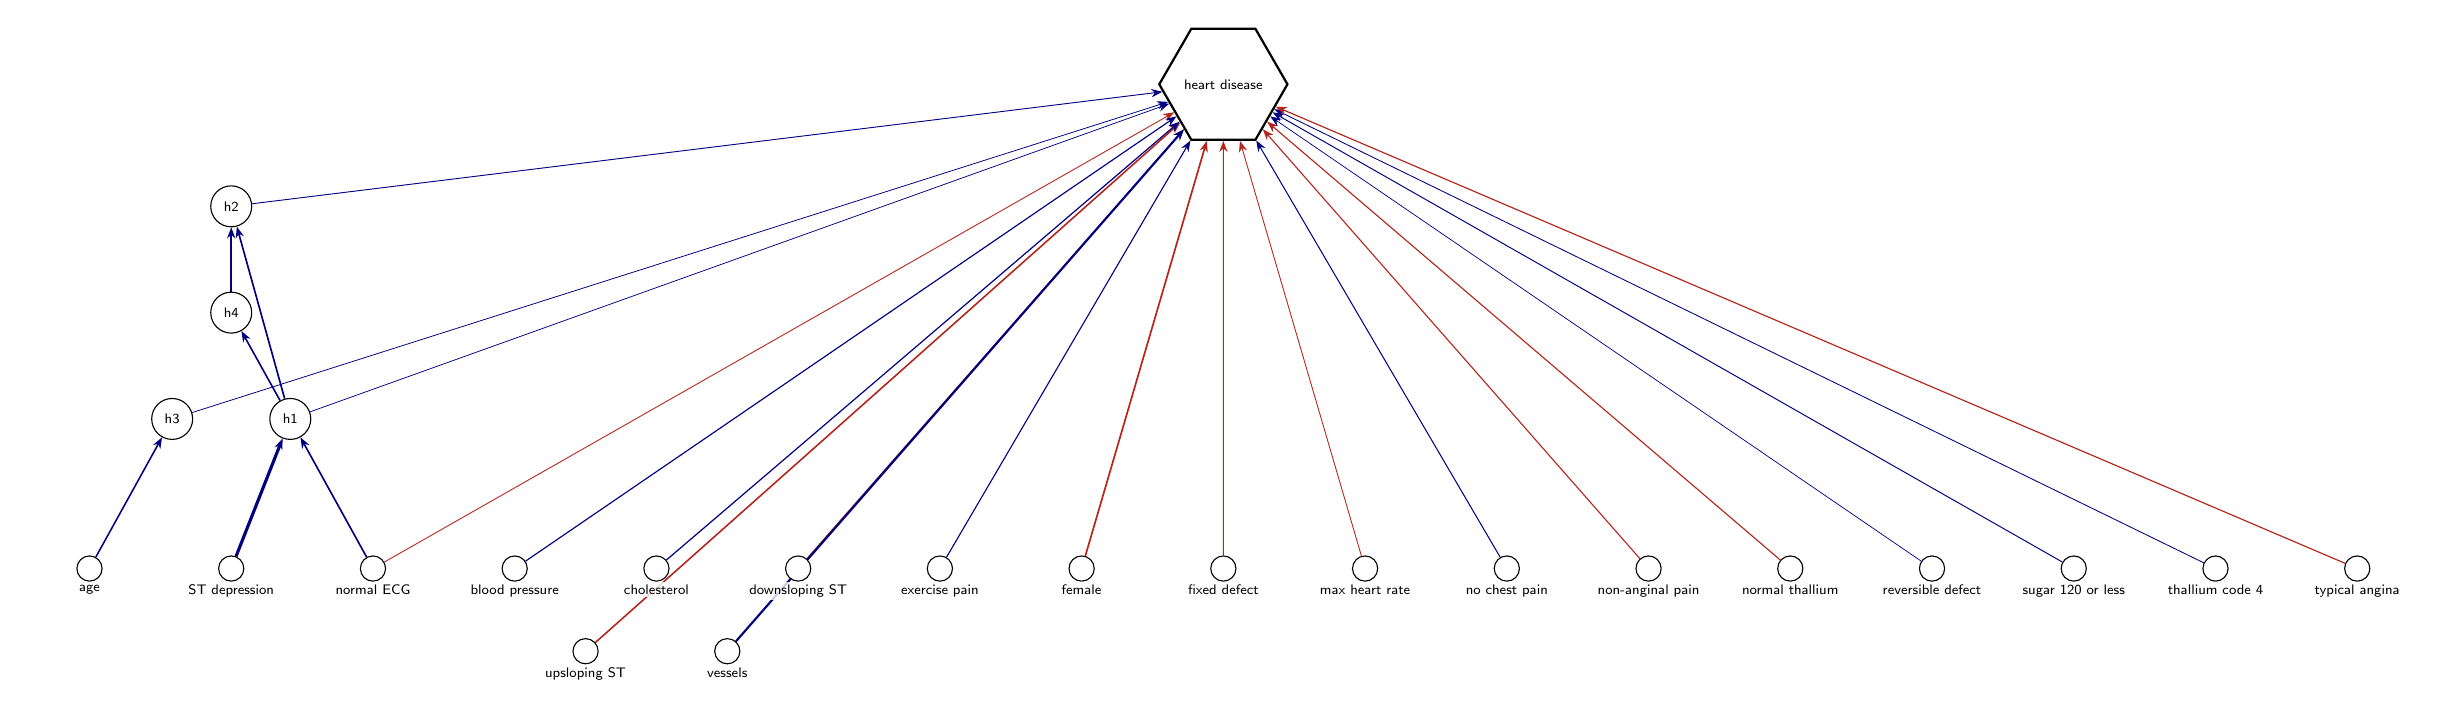
\begin{tikzpicture}[
  font=\sffamily\scriptsize, >={Stealth[length=1.4mm]},
  inp/.style={draw, circle, fill=white, minimum size=3.2mm, inner sep=0pt},
  hid/.style={draw, circle, fill=white, minimum size=5.2mm, inner sep=0.5pt, font=\sffamily\tiny},
  exitbox/.style={draw, thick, rectangle, fill=white, align=center, text width=17mm, minimum height=5mm, inner sep=1.5pt, font=\sffamily\tiny},
  sumbox/.style={draw, thick, dashed, rectangle, fill=white, align=center, text width=17mm, minimum height=5mm, inner sep=1.5pt, font=\sffamily\tiny},
  outp/.style={draw, thick, regular polygon, regular polygon sides=6, fill=white, minimum size=10mm, inner sep=0pt, font=\sffamily\tiny, align=center},
  stub/.style={draw, dashed, rounded corners=2pt, fill=white, align=center, inner sep=2pt, font=\sffamily\tiny, text width=15mm},
  inlab/.style={font=\sffamily\tiny, align=center, text width=15mm, inner sep=1pt, fill=white, fill opacity=0.8, text opacity=1},
  wpos/.style={draw=NavyBlue}, wneg/.style={draw=BrickRed}, wagg/.style={draw=black!45, line width=1.2pt},
  wmix/.style={draw=Plum},
]
\node[inp] (ninxxage) at (0.0,0.0) {};
\path (ninxxage.south) node[inlab, anchor=north] (labninxxage) {age};
\node[inp] (ninxxfbsx0) at (25.2,0.0) {};
\path (ninxxfbsx0.south) node[inlab, anchor=north] (labninxxfbsx0) {sugar 120 or less};
\node[inp] (ninxxrestecgx0) at (3.6,0.0) {};
\path (ninxxrestecgx0.south) node[inlab, anchor=north] (labninxxrestecgx0) {normal ECG};
\node[inp] (ninxxthalach) at (16.2,0.0) {};
\path (ninxxthalach.south) node[inlab, anchor=north] (labninxxthalach) {max heart rate};
\node[inp] (ninxxexangx1) at (10.8,0.0) {};
\path (ninxxexangx1.south) node[inlab, anchor=north] (labninxxexangx1) {exercise pain};
\node[inp] (ninxxoldpeak) at (1.8,0.0) {};
\path (ninxxoldpeak.south) node[inlab, anchor=north] (labninxxoldpeak) {ST depression};
\node[inp] (ninxxslopex1) at (6.3,-1.05) {};
\path (ninxxslopex1.south) node[inlab, anchor=north] (labninxxslopex1) {upsloping ST};
\node[inp] (ninxxsexx0) at (12.6,0.0) {};
\path (ninxxsexx0.south) node[inlab, anchor=north] (labninxxsexx0) {female};
\node[inp] (ninxxslopex3) at (9.0,0.0) {};
\path (ninxxslopex3.south) node[inlab, anchor=north] (labninxxslopex3) {downsloping ST};
\node[inp] (ninxxca) at (8.1,-1.05) {};
\path (ninxxca.south) node[inlab, anchor=north] (labninxxca) {vessels};
\node[inp] (ninxxthalx3) at (21.6,0.0) {};
\path (ninxxthalx3.south) node[inlab, anchor=north] (labninxxthalx3) {normal thallium};
\node[inp] (ninxxthalx4) at (27.0,0.0) {};
\path (ninxxthalx4.south) node[inlab, anchor=north] (labninxxthalx4) {thallium code 4};
\node[inp] (ninxxthalx6) at (14.4,0.0) {};
\path (ninxxthalx6.south) node[inlab, anchor=north] (labninxxthalx6) {fixed defect};
\node[inp] (ninxxthalx7) at (23.4,0.0) {};
\path (ninxxthalx7.south) node[inlab, anchor=north] (labninxxthalx7) {reversible defect};
\node[inp] (ninxxcpx1) at (28.8,0.0) {};
\path (ninxxcpx1.south) node[inlab, anchor=north] (labninxxcpx1) {typical angina};
\node[inp] (ninxxcpx3) at (19.8,0.0) {};
\path (ninxxcpx3.south) node[inlab, anchor=north] (labninxxcpx3) {non-anginal pain};
\node[inp] (ninxxcpx4) at (18.0,0.0) {};
\path (ninxxcpx4.south) node[inlab, anchor=north] (labninxxcpx4) {no chest pain};
\node[inp] (ninxxtrestbps) at (5.4,0.0) {};
\path (ninxxtrestbps.south) node[inlab, anchor=north] (labninxxtrestbps) {blood pressure};
\node[inp] (ninxxchol) at (7.2,0.0) {};
\path (ninxxchol.south) node[inlab, anchor=north] (labninxxchol) {cholesterol};
\node[outp] (n0) at (14.4,6.15) {heart disease};
\node[hid] (n1987) at (1.05,1.9) {h3};
\node[hid] (n204) at (2.55,1.9) {h1};
\node[hid] (n290) at (1.8,4.6) {h2};
\node[hid] (n3487) at (1.8,3.25) {h4};
\begin{scope}[on background layer]
\draw[->, wpos, line width=0.56pt] (ninxxage) -- (n1987);
\draw[->, wpos, line width=0.35pt] (ninxxfbsx0) -- (n0);
\draw[->, wneg, line width=0.32pt] (ninxxrestecgx0) -- (n0);
\draw[->, wpos, line width=0.59pt] (ninxxrestecgx0) -- (n204);
\draw[->, wneg, line width=0.32pt] (ninxxthalach) -- (n0);
\draw[->, wpos, line width=0.40pt] (ninxxexangx1) -- (n0);
\draw[->, wpos, line width=1.13pt] (ninxxoldpeak) -- (n204);
\draw[->, wneg, line width=0.56pt] (ninxxslopex1) -- (n0);
\draw[->, wneg, line width=0.61pt] (ninxxsexx0) -- (n0);
\draw[->, wneg, line width=0.40pt] (ninxxslopex3) -- (n0);
\draw[->, wpos, line width=0.77pt] (ninxxca) -- (n0);
\draw[->, wneg, line width=0.41pt] (ninxxthalx3) -- (n0);
\draw[->, wpos, line width=0.31pt] (ninxxthalx4) -- (n0);
\draw[->, wneg, line width=0.40pt] (ninxxthalx6) -- (n0);
\draw[->, wpos, line width=0.26pt] (ninxxthalx7) -- (n0);
\draw[->, wneg, line width=0.42pt] (ninxxcpx1) -- (n0);
\draw[->, wneg, line width=0.40pt] (ninxxcpx3) -- (n0);
\draw[->, wpos, line width=0.37pt] (ninxxcpx4) -- (n0);
\draw[->, wpos, line width=0.42pt] (ninxxtrestbps) -- (n0);
\draw[->, wpos, line width=0.44pt] (ninxxchol) -- (n0);
\draw[->, wpos, line width=0.28pt] (n1987) -- (n0);
\draw[->, wpos, line width=0.27pt] (n204) -- (n0);
\draw[->, wpos, line width=0.60pt] (n204) -- (n290);
\draw[->, wpos, line width=0.58pt] (n204) -- (n3487);
\draw[->, wpos, line width=0.33pt] (n290) -- (n0);
\draw[->, wpos, line width=0.55pt] (n3487) -- (n290);
\end{scope}
\end{tikzpicture}}%
\caption{The network as trained, before any explanation, in full. Blue: positive weight (raises the score); red: negative weight (lowers it); thicker: larger weight. Orange outline and up arrow: raises the final prediction; teal and down arrow: lowers it; grey and double arrow: depends. Not used (no connection): male, atypical angina, sugar above 120, ST-T abnormal ECG, LVH on ECG, no exercise pain, flat ST.}
\label{fig:hearts5c3:raw}
\end{figure}
\end{landscape}
\end{drafted}
\clearpage
\end{document}
